\markedchapter{Non-orientable WSMs}{Non-orientability and Weyl points}\label{chap:non-orientable}

Symmetries play a crucial role in establishing and differentiating topological properties of physical systems; this is attested by the tenfold way classification discussed in Section \ref{sec:symm-classes}. However, in recent years researchers have begun to recognise that symmetries beyond the standard time reversal, charge conjugation and chiral symmetries can give rise to distinct topological invariants that are not fully captured by this classification.

An important class of these extended symmetries is comprised by the space groups acting on periodic lattices. These impose additional structure on the unit cell of the lattice, such as rotational or reflection symmetry. The space groups may induce novel topological states when applied to a material lattice \cite{Po_space-groups}; the classification of these states is covered exhaustively in Ref.~\cite{Shiozaki_AHSS}. Of special interest in this work are the so-called \emph{non-symmorphic} space group symmetries, which combine basic rotation, reflection or inversion with fractional lattice translations. This type of symmetry features fewer high-symmetry points, and its effect on real-space lattices has been studied extensively \cite{Wang_hourglass,Chen_nonsymmorphic-semimetal,Kim_glide-semimetal,Shiozaki_nonsymmorphic-topology,Bzdusek_nodal-chain,Wieder_layer-semimetal,Zhao_nonsymmorphic-semimetal,Yang_nonsymmorphic-semimetal,Wang_hourglass-semimetal,Wang_hourglass-Dirac,Wieder_wallpaper-fermions,Xiao_hourglass-Weyl}; a review can be found at Ref.~\cite{Zhang_nonsymmorphic-review}.

Very recently, the feasibility of applying these non-symmorphic symmetries in momentum space has been demonstrated both theoretically and experimentally \cite{CYZ_Klein-gauge,Zhang_nonsymmorphic,TaoYan_acoustic-Klein,Zhu_acoustic-Klein-halfturn,HZY_RP2,WangZhang_acoustic-Klein-2D,Tao_quadrupole,Fonseca-Vaidya_nonorientable,KönigYang_nonorientable-EPs}. This opens up new and interesting avenues of research relating to Brillouin zone topology. In particular, the Brillouin zone may become effectively non-orientable, challenging the notion of chirality for Weyl points.

We begin this chapter with a short review of existing literature surrounding these momentum-space non-symmorphic symmetries in Section~\ref{sec:review}, culminating in a treatment of a recent paper which applies them to Weyl semimetals. We then present a novel topological analysis of the system described in this paper in Section~\ref{sec:non-ori_topology}, in terms of the cohomology and homology tools presented in Chapter~\ref{chap:WSM}. We also develop a formalism for studying and interpreting semimetal invariants in a more general non-orientable setting. In Section~\ref{sec:non-ori_classification}, we provide a full classification of all possible non-orientable Brillouin zones in three dimensions, including explicit calculations of the semimetal Mayer--Vietoris sequence for each one. Finally, in Section~\ref{sec:inversion}, we apply the insights gained from these non-orientable systems to the important case of inversion-symmetric Weyl semimetals. Using a heuristic ansatz, we derive a semimetal Mayer--Vietoris sequence that appears to correctly classify the topological invariants of these systems.


\markedsection{Review}{Review of recent literature}\label{sec:review}

Non-symmorphic symmetries have been studied somewhat extensively in real space, but their momentum space counterparts have long eluded study. There is a practical reason for this: normally, any space group symmetry in real space gives rise to a symmorphic (i.e.\ point group) symmetry in momentum space after Fourier transformation, regardless of the nature of the real space symmetry \cite{Zhang_nonsymmorphic}. In order to obtain a non-symmorphic symmetry in momentum space, it is necessary to change how the real-space symmetry group acts on states in the Hilbert space. The reasoning is as follows: a symmetry group $G$ acts on states in the Hilbert space through a representation $\rho$. This representation is normally a homomorphism, i.e.\ it obeys
\begin{equation*}
	\rho(g)\rho(h) = \rho(gh)
\end{equation*}
for $g,h\in G$. However, since quantum states are physically equivalent up to a $\U(1)$ phase, the representation $\rho$ may also include $\U(1)$ factors:
\begin{equation*}
	\rho(g)\rho(h) = \nu(g,h)\rho(gh),
\end{equation*}
where $\nu: G\times G\to \U(1)$ is known as a factor system \cite{Chen_gauge-classification}. Such a representation is called \emph{projective}, and it may fundamentally alter the algebraic properties of the symmetry group---for example, it can lead symmetry operations that commute in real space to anticommute instead in Hilbert space. Projective representations have previously been studied in more abstract systems, and may give rise to novel topological phases on their own \cite{ZHY_Z2-projective,Zhao_projective-PT,Shao_gauge,Xue-Wang_acoustic-Mobius,Li-Du_acoustic-Mobius,Chen_gauge-classification}. The usual strategy is to implement \emph{gauge fluxes} on the real-space lattice; these are structures that induce $\U(1)$ phase changes in particles hopping around the lattice.

The first theoretical realisation of non-symmorphic momentum space symmetries was published by Z.~Y.~Chen, Shengyuan Yang and Yuxin Zhao in 2022 \cite{CYZ_Klein-gauge}. In their work, the authors take a lattice with a mirror symmetry $M_x$ and perpendicular translation symmetry $L_y$, and demonstrate how negative hopping amplitudes may be implemented in such a way that the resulting gauge fluxes make $M_x$ and $L_y$ anticommute rather than commute; see Figure \ref{subfig:gauge-flux}.
\begin{figure}[htb!]
	\centering
	\subcaptionbox{\label{subfig:gauge-flux}}{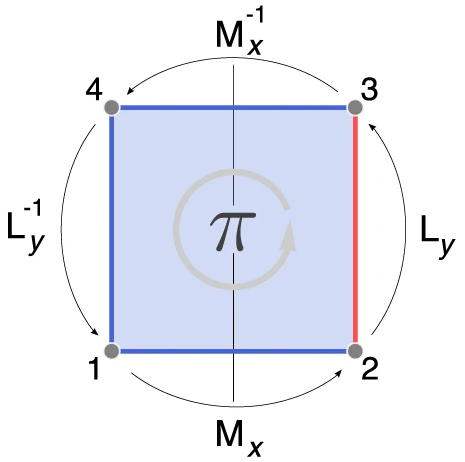
\includegraphics[width=.28\linewidth]{Images/Gauge-flux}}
	\hfil
	\subcaptionbox{\label{subfig:Klein-BZ}}{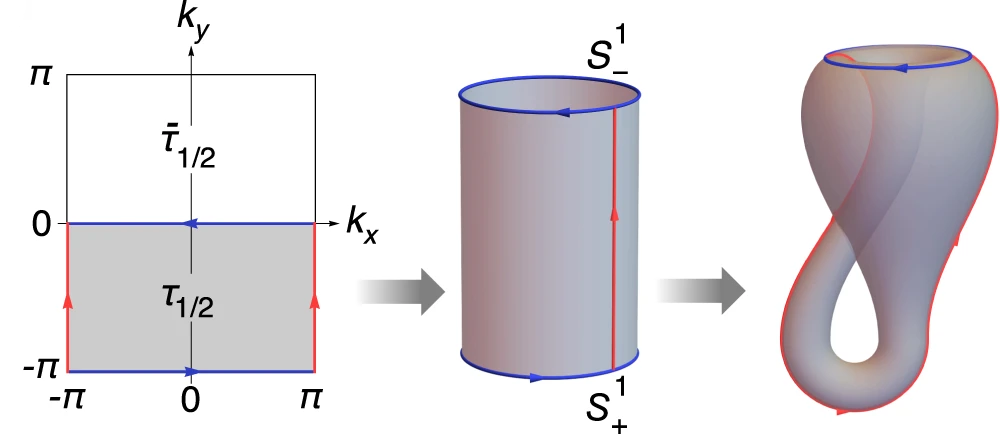
\includegraphics[width=.62\linewidth]{Images/Klein-BZ}}
	\caption{Figures adapted from Ref.~\cite{CYZ_Klein-gauge}. (a) A square section of the lattice is shown with a negative hopping amplitude in red. This induces a phase change of $\pi$ (i.e.\ a sign change) on a test particle which is moved around the square by successive symmetry operations $L_y^{-1}M_x^{-1}L_yM_x$. The operators $M_x$ and $L_y$ anticommute as a result. (b) The momentum space symmetry $\hat{M}_x$ reduces the Brillouin torus to the fundamental domain shaded in grey on the left. The boundaries of this domain are identified along the red and blue arrows, upon which it assumes the topology of the Klein bottle $K^2$ (shown on the right). Much like a Möbius strip, this surface has only one side: in the illustration, the outside of the main bulb is connected to its inside via the funnel at the top. This means $K^2$ cannot be given a consistent orientation.}
	\label{fig:CYZ_Klein}
\end{figure}
This anticommutation changes how the mirror operator acts in momentum space: denoting the momentum space operators by $\hat{M}_x$ and $\hat{L}_y=\e^{ik_y}$ (assuming unit lattice spacing in the real $y$ direction), anticommutation implies
\begin{equation*}
	\hat{M}_x\e^{ik_y}\hat{M}_x = -\e^{ik_y} = \e^{i(k_y+\pi)}.
\end{equation*}
That is, $\hat{M}_x$ induces not only a mirroring $k_x\mapsto-k_x$, but also a translation by $\pi$ in the $k_y$ direction. It follows that the momentum-space Hamiltonian must obey the \emph{glide symmetry}
\begin{equation}\label{eq:2D_glide}
	U\Hc(k_x, k_y)U^{-1} = \Hc(-k_x, k_y + \pi).
\end{equation}
Crucially, the action of this symmetry is free, i.e.\ there are no high-symmetry momenta that are fixed by $\hat{M}_x$. Similar to the way in which the free $\Z^2$ translation symmetries on the 2D lattice reduce momentum space from $\R^2$ down to the Brillouin torus $\T^2$, this free $\Z_2$ glide symmetry reduces the Brillouin zone further down to a \emph{fundamental domain} covering half of the torus from $k_y=-\pi$ to $k_y=0$. Whereas the boundary conditions on the full torus are periodic, this fundamental domain features anti-periodic boundary conditions in the $k_y$ direction, in the sense that the $k_y=-\pi$ and $k_y=0$ boundaries must be identified with opposite orientations. Under these identifications, the fundamental domain assumes the topology of the Klein bottle $K^2$, which is a non-orientable surface; see Figure~\ref{subfig:Klein-BZ}.\footnote{
	Incidentally, Figure~\ref{subfig:Klein-BZ} serves as the inspiration for the cover page of this thesis.}

A note on terminology is in order here: the fundamental domain is an instance of an effective Brillouin zone as we have defined it in Section~\ref{sec:T-WSMs}, i.e.\ the quotient of the torus by the symmetry group. We use the more specific term ``fundamental domain'' to indicate that this region can be considered a true Brillouin zone in the absence of high-symmetry points. In this light, we avoid using the term ``Brillouin zone'' in isolation from here on to avoid confusion between the original Brillouin torus and this fundamental domain.

Returning to Ref.~\cite{CYZ_Klein-gauge}, the glide symmetric system is found to feature a $\Z_2$ invariant $\nu$, different from the $\Z$ invariant on the 2D Chern insulators discussed in Section~\ref{sec:Chern}. The difference may be explained in terms of cohomology: the regular Chern number is related to $H^2(\T^2)\cong\Z$, whereas in the case of the Klein bottle, the invariant is classified by $H^2(K^2)\cong\Z_2$. This $\Z_2$ invariant cannot be stated simply in terms of a Berry curvature integral on the fundamental domain: the boundaries at $k_y=-\pi$ and $k_y=0$ are identified in opposite directions, and their contributions to the integral no longer cancel by Stokes' theorem. Instead, the invariant takes the following two forms in Ref.~\cite{CYZ_Klein-gauge}:
\begin{align}
	\nu &\equiv \frac{1}{2\pi}\int_{\tau_{1/2}}\!\!\Fc + \frac{1}{\pi}\gamma(0) \mod 2 \label{eq:z2-inv1} \\
		&\equiv \frac{1}{2\pi}[\gamma(0) + \gamma(-\pi)]\mod 2, \label{eq:z2-inv2}
\end{align}
where $\tau_{1/2}$ is the fundamental domain and $\gamma(k_y)$ is the Berry phase over the loop at $k_y$. These two forms are related by Stokes' theorem, and the modulus 2 is necessary to ensure gauge invariance.\footnote{
	Note that in the latter equation, it is important that $\gamma(0)$ and $\gamma(-\pi)$ are both calculated in the same gauge, which must be continuous across the fundamental domain $\tau_{1/2}$.}

In 2023, Chen Zhang et al.\ (including two of the authors of the aforementioned Klein bottle paper) generalised this theoretical framework \cite{Zhang_nonsymmorphic}. In particular, they specify how to obtain all 157 non-symmorphic symmetries in three dimensions (and all four in two dimensions) from real-space gauge symmetries.

Several experimental verifications of these momentum-space non-symmorphic symmetries were published in 2024: Ref.~\cite{TaoYan_acoustic-Klein} by Yu-Liang Tao, Mou Yan et al.\ and Ref.~\cite{Zhu_acoustic-Klein-halfturn} by Zhenxiao Zhu et al. In both works, a 3D acoustic lattice is constructed---an artificial crystal in which the band structure is represented by frequencies of sound waves---featuring negative hopping amplitudes, which induce non-symmorphic symmetries in momentum space; see Figure \ref{fig:acoustic-Klein}.
\begin{figure}[htb!]
	\centering
	\subcaptionbox{\label{subfig:acoustic-couplings}}{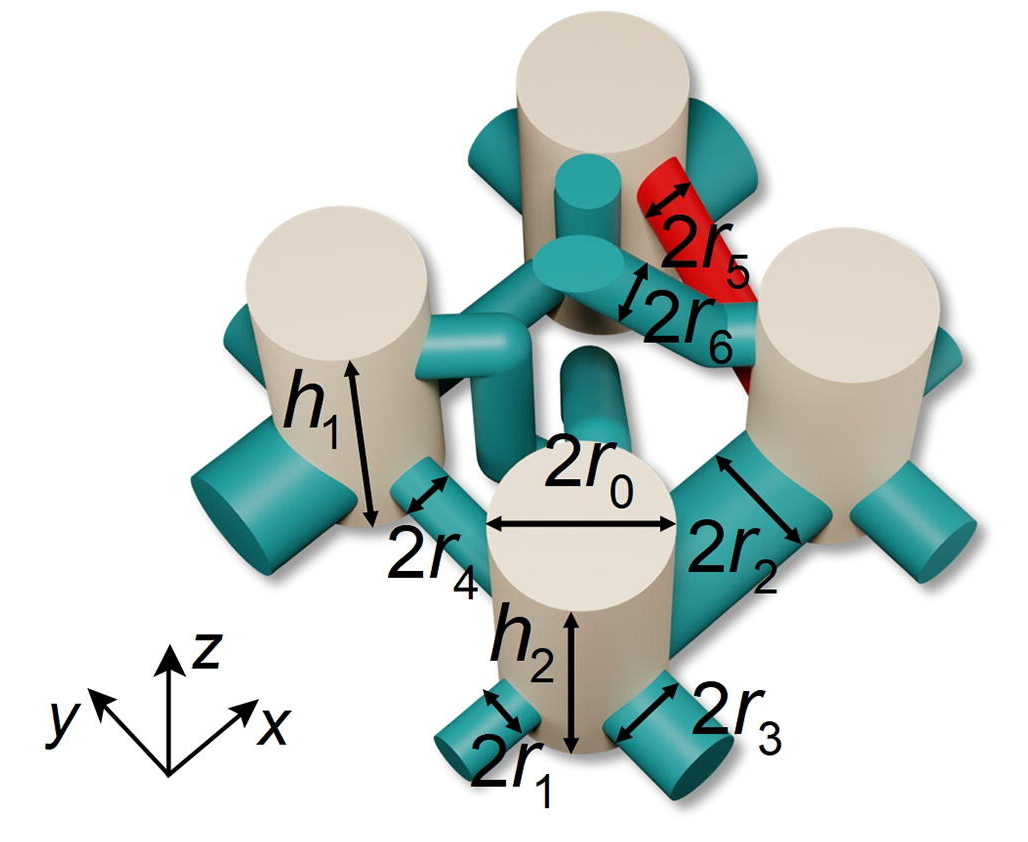
\includegraphics[width=.4\linewidth]{Images/acoustic-couplings}}
	\hfil
	\subcaptionbox{\label{subfig:acoustic-Klein}}{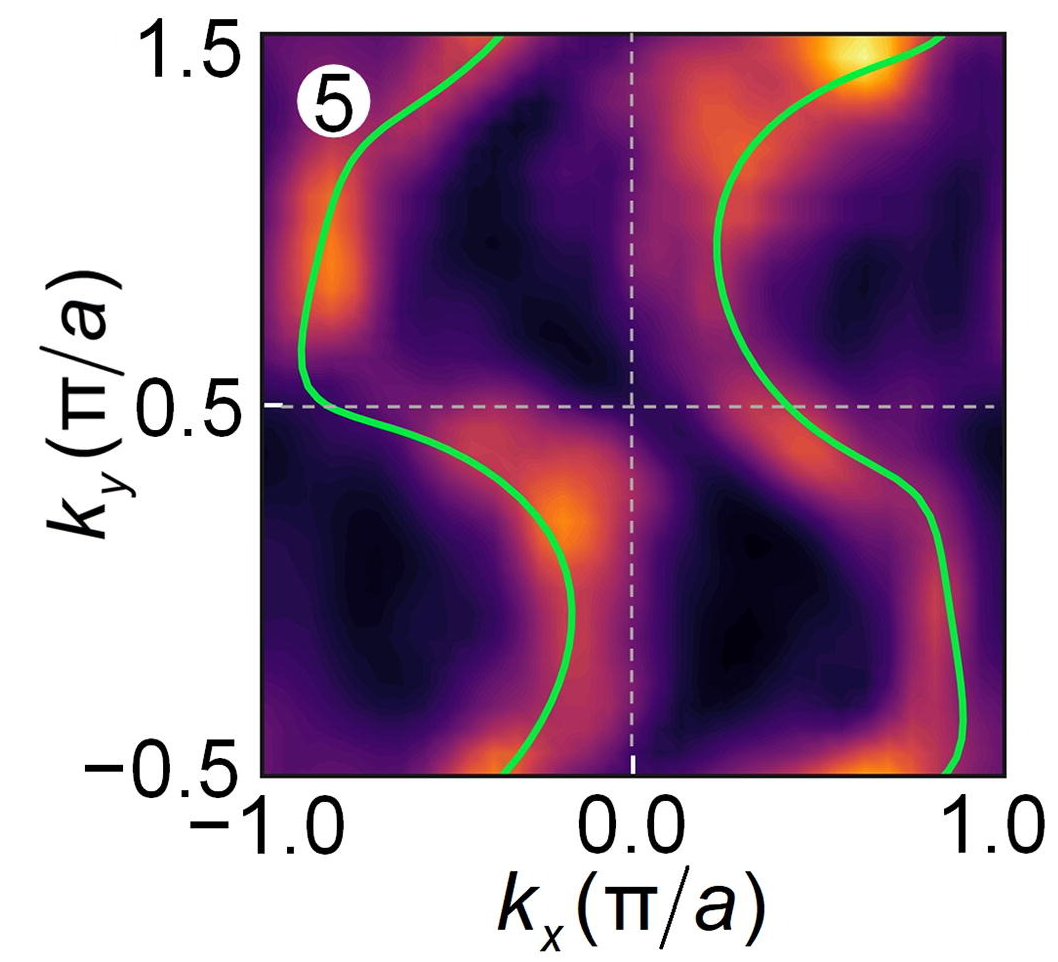
\includegraphics[width=.4\linewidth]{Images/acoustic-Klein}}
	\caption{Figure adapted	from Ref.~\cite{Zhu_acoustic-Klein-halfturn}. (a) Unit cell of the acoustic crystal used in the experiment. The resonant cavities shown in beige approximate tight-binding orbitals in electronic systems, while the coupling tubes in green simulate hopping between lattice sites. The tube indicated in red has an effective negative hopping amplitude. (b) Experimental (colour map) and numeric (green) data from a 2D slice of the system's Brillouin torus. The figure shows the response to a specific frequency, equivalent to an equal-energy contour (i.e. section of the bands) in an electronic system. This 2D slice features a glide symmetry: the lower half can be obtained by mirroring the upper half in the horizontal $k_x$ direction.}
	\label{fig:acoustic-Klein}
\end{figure}
These symmetries are shown to give rise to novel topological phases and surface behaviour.

Several other works have explored a specific non-symmorphic symmetry group in two dimensions, where besides the glide symmetry $\hat{M}_x$ giving rise to Equation \eqref{eq:2D_glide}, there is also a perpendicular glide symmetry $\hat{M}_y$ in which the roles of $k_x$ and $k_y$ are reversed \cite{HZY_RP2,WangZhang_acoustic-Klein-2D,Tao_quadrupole}. This double glide symmetry is notable in that, even though the action of each individual glide symmetry $\hat{M}_x$ and $\hat{M}_y$ on the Brillouin torus is free, the combined action of the two is not. Instead, there are four high-symmetry momenta\footnote{
	In crystallographic terms, the 2D wallpaper group Pgg has four special Wyckoff positions.}
at $\k = (\pm\pi/2,\pm\pi/2)$ which are fixed under $\hat{M}_y\hat{M}_x$; see Figure~\ref{fig:Pgg-fixed-points}.
\begin{figure}[htb!]
	\centering
	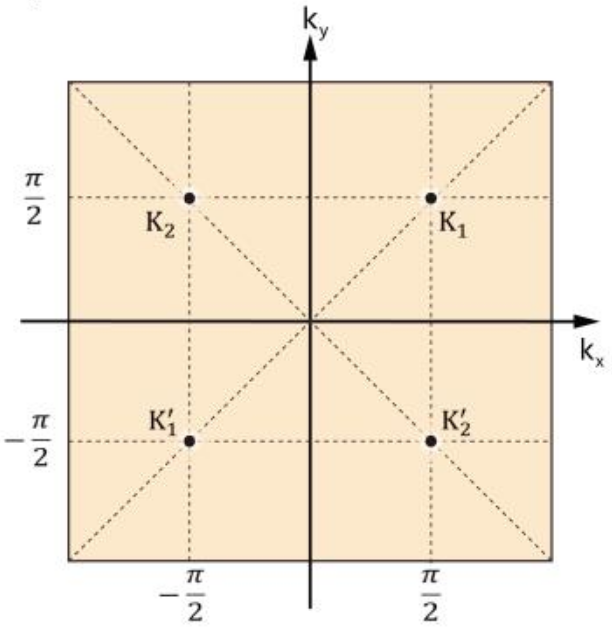
\includegraphics[width=.5\linewidth]{Images/Pgg-fixed-points}
	\caption{Figure from Ref.~\cite{WangZhang_acoustic-Klein-2D}. The points labelled $K_a$ with $a\in\{1,2\}$ are related by either single glide symmetry to those labelled $K_a'$ respectively. As a result, applying both symmetries at once fixes all four of these points. The indicated dashed lines are also fixed sets of the combined symmetry.}
	\label{fig:Pgg-fixed-points}
\end{figure}
It is noted in Refs.~\cite{HZY_RP2} and \cite{WangZhang_acoustic-Klein-2D} that a $\Z_2$ topological invariant can be calculated based on the eigenvalues of $\hat{M}_x\hat{M}_y$ at these high-symmetry points, similar to the $\Z_2$ invariants in the time-reversal invariant systems encountered in Section \ref{sec:insulators}.

\subsection{Non-orientable Weyl semimetals}

The first work in which non-symmorphic symmetries were explored in the context of Weyl semimetals was a 2024 paper by André Grossi Fonseca, Sachin Vaidya et al. \cite{Fonseca-Vaidya_nonorientable}. The remainder of this section is dedicated to summarizing the main findings in this paper.

The basic setup in Ref.~\cite{Fonseca-Vaidya_nonorientable} is that of an abstract 3D Brillouin torus featuring a glide symmetry of the form
\begin{equation}\label{eq:3D_glide}
	\Hc(k_x, k_y, k_z) = \Hc(-k_x, k_y + \pi, k_z);
\end{equation}
no assumptions are made on the source of this symmetry.\footnote{
	The symmetry is presented without unitary conjugation, but as noted in the supplement to Ref.~\cite{Fonseca-Vaidya_nonorientable}, the presence of such a conjugation [as in Equation~\eqref{eq:2D_glide}] makes no difference topologically.}
The free action of this symmetry gives rise to a non-orientable fundamental domain: slices of constant $k_z$ take on the topology of the Klein bottle $K^2$ in the same way as in Ref.~\cite{CYZ_Klein-gauge} discussed above. Taking into account the additional periodic $k_z$ direction, the total fundamental domain is topologically the non-orientable manifold $\KS$; see Figure~\ref{fig:K2S1}.
\begin{figure}[htb!]
	\centering
	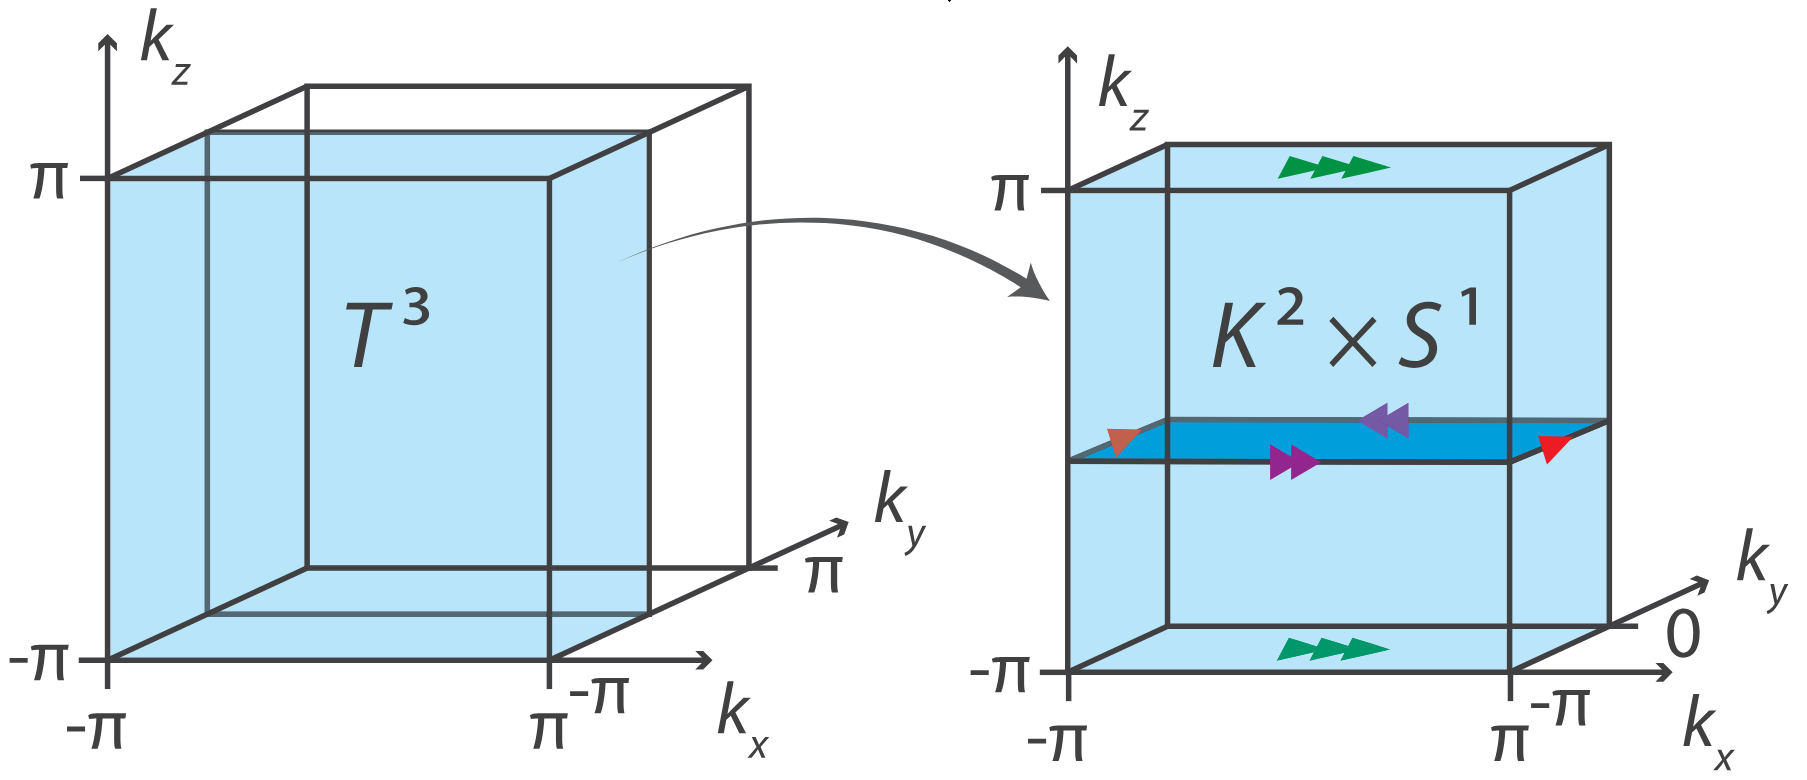
\includegraphics[width=.7\linewidth]{Images/K2S1}
	\caption{Figure adapted from Ref.~\cite{Fonseca-Vaidya_nonorientable}. The glide symmetry in Equation~\eqref{eq:3D_glide} acts on the Brillouin torus $\T^3$ in such a way that the fundamental domain (covering half the torus) is topologically $\KS$. Coloured arrows indicate the correct boundary identifications.}
	\label{fig:K2S1}
\end{figure}
In Ref.~\cite{Fonseca-Vaidya_nonorientable}, the fundamental domain is taken to be the half torus with $k_y\leq 0$, with additional boundary identifications between the planes $k_y=-\pi$ and $k_y=0$ which respect the symmetry.

The non-orientability of the fundamental domain is shown to lead to some novel properties. Most notably, the chirality of Weyl points is no longer well-defined in a non-orientable setting: for example, when a Weyl point which has a Chern number of $-1$ leaves the fundamental domain at the $k_y=-\pi$ plane, it returns at the corresponding point on the $k_y=0$ plane with a Chern number of $+1$. Physically, this is because the glide symmetry in Equation~\eqref{eq:3D_glide} is parity-reversing, which induces a sign change in the Berry curvature.

These chirality changes may result in a system in which the total chirality of Weyl points does not add to zero on the fundamental domain; that is, the Nielsen--Ninomiya charge cancellation theorem in Equation~\eqref{eq:Nielsen-Ninomiya} is circumvented. In particular, two Weyl points with the same chirality may be connected by a Fermi arc on an $xy$-like surface, see Figure~\ref{fig:same-chirality}.
\begin{figure}[htb!]
	\centering
	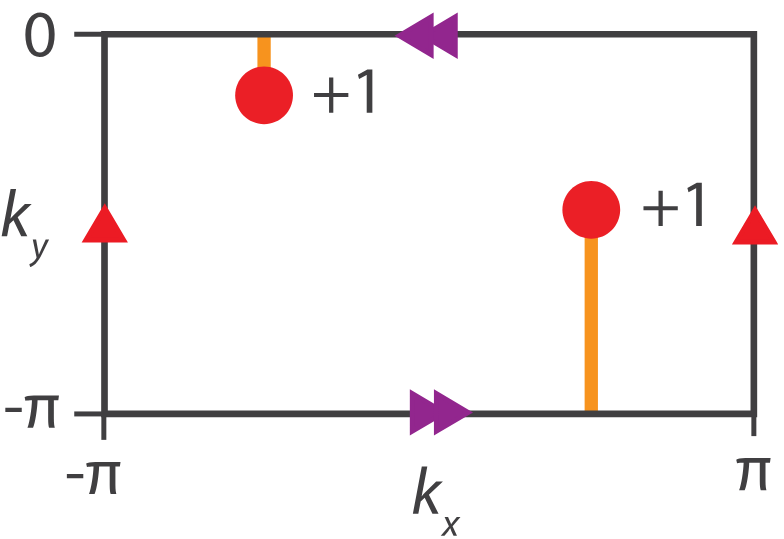
\includegraphics[width=.5\linewidth]{Images/same-chirality}
	\caption{Figure from Ref.~\cite{Fonseca-Vaidya_nonorientable}. Surface Brillouin zone obtained from imposing open boundary conditions in the $z$ direction. A Fermi arc is shown which connects (projections of) Weyl points of the same chirality. This Fermi arc crosses the orientation-reversing boundary at $k_y=0$ once (i.e.\ an odd number of times).}
	\label{fig:same-chirality}
\end{figure}
It is demonstrated that a Fermi arc on such a surface connects two same-chirality Weyl points if and only if it lies on an ``orientation-reversing path'', i.e.\ it crosses the line at $k_y=0$ an odd number of times.

Moreover, a new charge cancellation theorem is derived from a $\Z_2$ invariant $\nu$ existing on gapped $K^2$-like slices of constant $k_z$. This invariant is equivalent to that on the Klein bottle insulator in Ref.~\cite{CYZ_Klein-gauge}, and is calculated using Equations~\eqref{eq:z2-inv1} and \eqref{eq:z2-inv2}. It is shown that this invariant changes whenever such a slice is moved across a Weyl point of odd chirality in the $k_z$ direction, see Figure \ref{fig:Z2-cancellation}.
\begin{figure}[htb!]
	\centering
	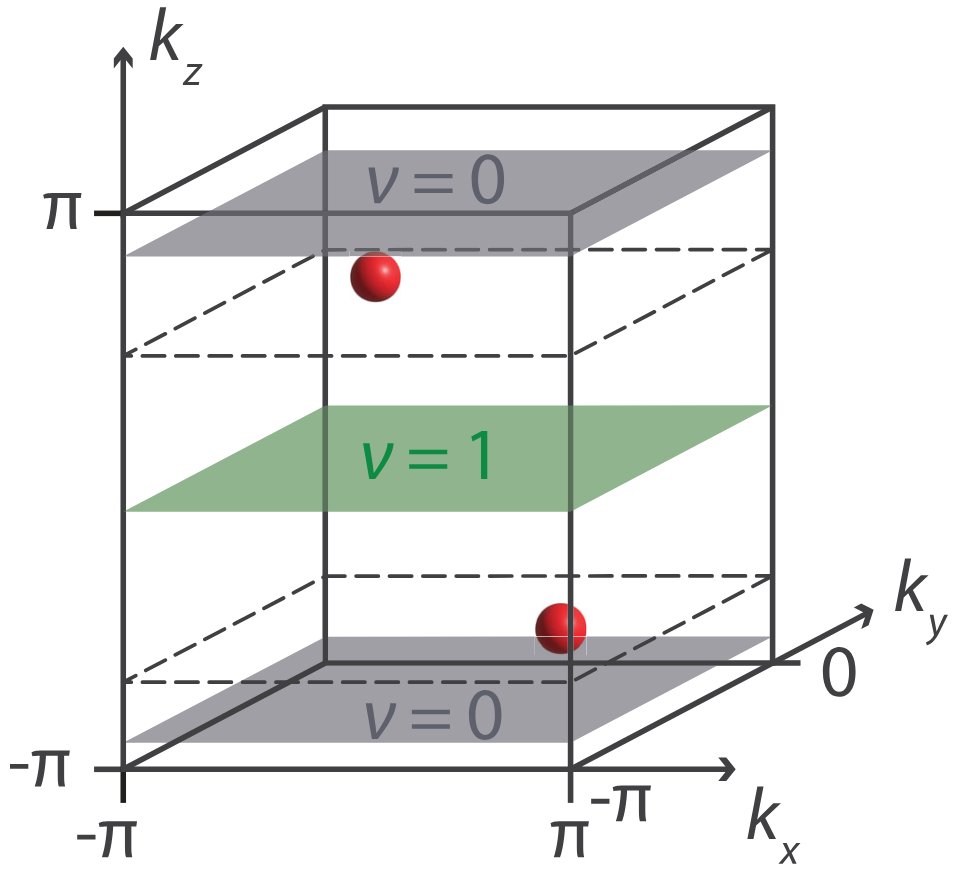
\includegraphics[width=.5\linewidth]{Images/Z2-cancellation}
	\caption{Figure from Ref.~\cite{Fonseca-Vaidya_nonorientable}. The $\KS$ fundamental domain is shown featuring two Weyl points, both with chirality $+1$. The invariant $\nu$ is shown to vary in the $k_z$ direction, depending on the presence of Weyl points. Periodicity in the $k_z$ direction then dictates that the total parity of the Weyl points must be even.}
	\label{fig:Z2-cancellation}
\end{figure}
It is then argued that, since the fundamental domain is periodic in the $k_z$ direction, there must be an even number of such changes in $\nu$. This leads to a novel $\Z_2$ charge cancellation condition for Weyl points on $\KS$: if there are $k$ Weyl points $w_i\in W$ in the fundamental domain, then their Chern numbers $C_{w_i}$ must obey
\begin{equation}\label{eq:Z2-cancellation}
	\sum_{i=1}^{k}C_{w_i} = 0 \mod 2.
\end{equation}

Finally, Ref.~\cite{Fonseca-Vaidya_nonorientable} includes an experimental realisation of a Weyl semimetal with momentum-space glide symmetry. The authors make use of one-dimensional photonic crystals, whose longitudinal coordinate $z$ represents the $z$ direction inside a three-dimensional semimetal. The optical properties of the unit cells of each crystal are parametrised by two periodic variables $k_1$ and $k_2$, which effectively act as synthetic versions of the momenta $k_x$ and $k_y$. These synthetic momenta are made to obey the glide symmetry in Equation~\eqref{eq:3D_glide}, in such a way that the resulting system acts like a Weyl semimetal with two Weyl points of equal chirality in the fundamental domain. The optical crystals are then truncated in the $z$ direction, so that surface states on the $K^2$-like $(k_x,k_y)$ surface may be probed at specific momenta. In this way, a Fermi arc is demonstrated which terminates in two points of similar chiralities; see Figure~\ref{fig:K2-experiment}.
\begin{figure}[htb!]
	\centering
	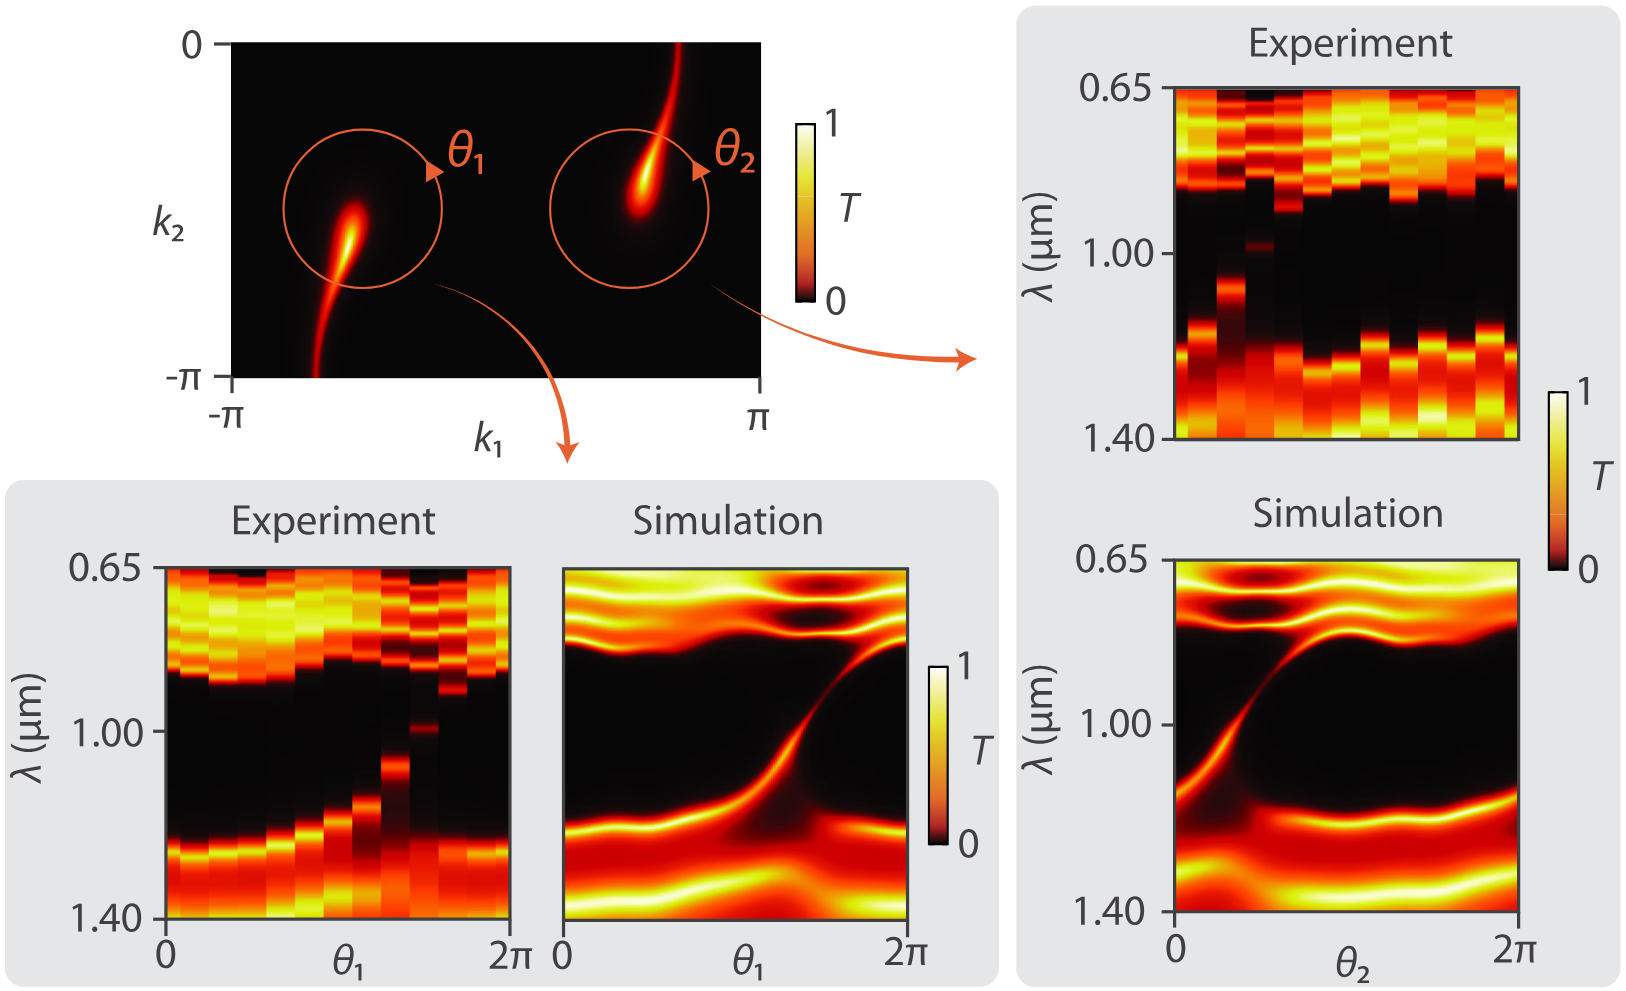
\includegraphics[width=.9\linewidth]{Images/K2-experiment}
	\caption{Figure from Ref.~\cite{Fonseca-Vaidya_nonorientable}. Top left: simulated $K^2$ surface Brillouin zone featuring a Fermi arc that crosses the orientation-reversing boundary at $k_2=-\pi\sim 0$. Two circular contours are shown, parametrised by $\theta_1$ and $\theta_2$. Bottom left: experimental (photonic) samples are prepared for several discrete values of $\theta_1$, with their synthetic momenta matched to the $(k_1,k_2)$ corresponding to $\theta_1$. The plots show the frequency response (i.e.\ band structure) on the surface Brillouin zone as $\theta_1$ runs from $0$ to $2\pi$. The rising dispersion indicates a positive chirality of the underlying Weyl point. Right: Similar samples are prepared for values of $\theta_2$. The dispersion is also ascending here, indicating a second positively charged Weyl node.}
	\label{fig:K2-experiment}
\end{figure}


\markedsection{Topology}{Topological exploration}\label{sec:non-ori_topology}

The purpose of this section is to reframe and analyse the non-orientable Weyl semimetals described in Ref.~\cite{Fonseca-Vaidya_nonorientable} in terms of the algebraic topology language from Chapter \ref{chap:WSM}. This approach has the advantage of being coordinate-free, and as such it provides a more fundamental understanding of the system's topological properties. We obtain a direct description of how the Nielsen--Ninomiya theorem is modified into the $\Z_2$ charge cancellation condition in Equation~\eqref{eq:Z2-cancellation}. We also obtain a more complete picture of the different invariants associated with such a system, and are able to distinguish which are related to the topological insulator phase, and which relate to the introduction of Weyl nodes. Along the way, we develop a formalism for studying semimetal topology in a more general non-orientable setting. To the knowledge of the author, the insights contained in the remainder of this chapter are novel.

\subsection{Preliminary clarifications}\label{sec:clarifications}

As a motivation for the proposed coordinate-free description, we begin by elucidating some minor points of confusion present in Ref.~\cite{Fonseca-Vaidya_nonorientable}.

First of all, there is a relatively strong emphasis on the two ``orientation-reversing planes'' at $k_y=\pm\pi$ and $k_y=0$. For example, it is stated that relative chirality can be defined unambiguously on fundamental domains that avoid these planes. This is true on a technical level, but it creates the impression that the orientation reversal occurs locally at the boundary of the fundamental domain, raising questions about the nature of Weyl points existing on these planes.

In reality, orientation reversal is a global feature. We are free to reparametrise the fundamental domain in a way that includes the planes $k_y=\pm\pi$ and $k_y=0$, and the notion of relative chirality may change as a result; this is illustrated in Figure~\ref{fig:BZ_param}.
\begin{figure}[htb!]
	\centering
	\subcaptionbox{$-\pi \leq k_y \leq 0$\label{subfig:BZ_basic}} {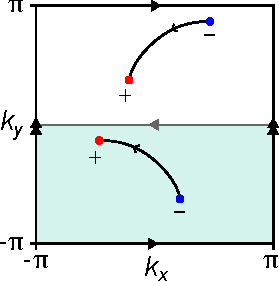
\includegraphics[width=.3\textwidth]{Images/BZ_basic}}
	\hfil
	\subcaptionbox{$-\pi/2 \leq k_y \leq \pi/2$}{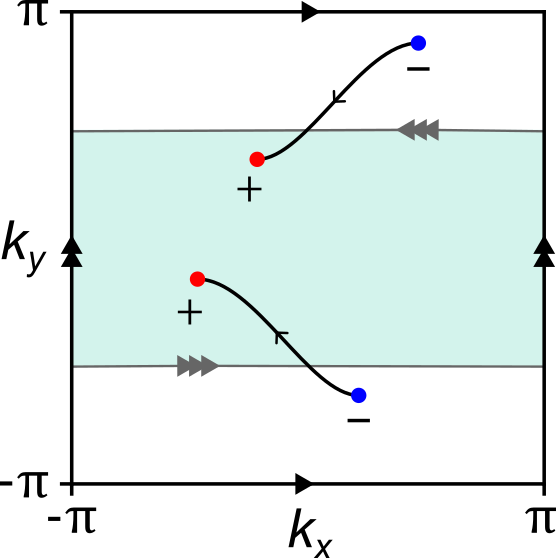
\includegraphics[width=.3\textwidth]{Images/BZ_mid}}
	\hfil
	\subcaptionbox{$0 \leq k_x \leq \pi$\label{subfig:BZ_right}} {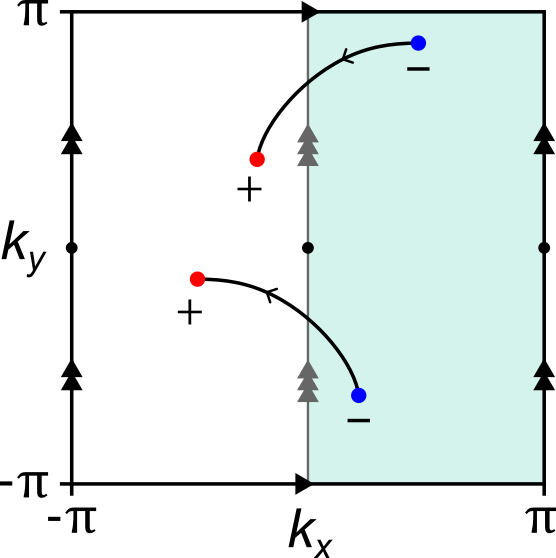
\includegraphics[width=.3\textwidth]{Images/BZ_right}}
	\caption{Top view of the 3D Brillouin torus (or 2D surface torus) for a given Weyl semimetal state obeying the glide symmetry in Equation~\eqref{eq:3D_glide}, with Weyl points and oriented Dirac strings (Fermi arcs) drawn in. Different parametrisations of the fundamental domain are shaded in teal: (a) the domain outlined in Ref.~\cite{Fonseca-Vaidya_nonorientable}; (b) the same domain shifted in the $k_y$ direction; (c) a domain spanning the $k_y$ direction. Each of these domains is homeomorphic to $\KS$ ($K^2$) under the boundary identifications shown. Note that both the absolute and relative chirality of the two Weyl nodes in the fundamental domain change under these alternative parametrisations.}
	\label{fig:BZ_param}
\end{figure}
For any given set of distinct Weyl points obeying the symmetry, it is possible in principle to achieve any relative chirality by reparametrising the fundamental domain. It should be noted that there do exist two planes that are of special significance, namely the so-called \emph{glide planes} at $k_x = 0$ and $k_x = \pm\pi$; these planes are (taken as a whole) invariant under the symmetry, and as such they cannot be excluded completely from any given parametrisation.

A similar point of confusion arises in explaining how the usual relation between Nielsen--Ninomiya and the Poincaré--Hopf theorem for vector fields breaks down. On the regular Brillouin torus, the factor $\h(\k)$ in the Bloch Hamiltonian can be considered a continuous vector field tangent to the torus. The Poincaré--Hopf theorem then tells us that the zeroes of such vector fields must have topological indices (corresponding to Weyl point chiralities) adding up to zero.

In the supplement to Ref.~\cite{Fonseca-Vaidya_nonorientable}, the failure of Poincaré--Hopf is attributed to a discontinuity of the vector field at the planes $k_y=\pm\pi$ and $k_y=0$; see Figure~\ref{fig:Klein-discontinuity}.
\begin{figure}[htb!]
	\centering
	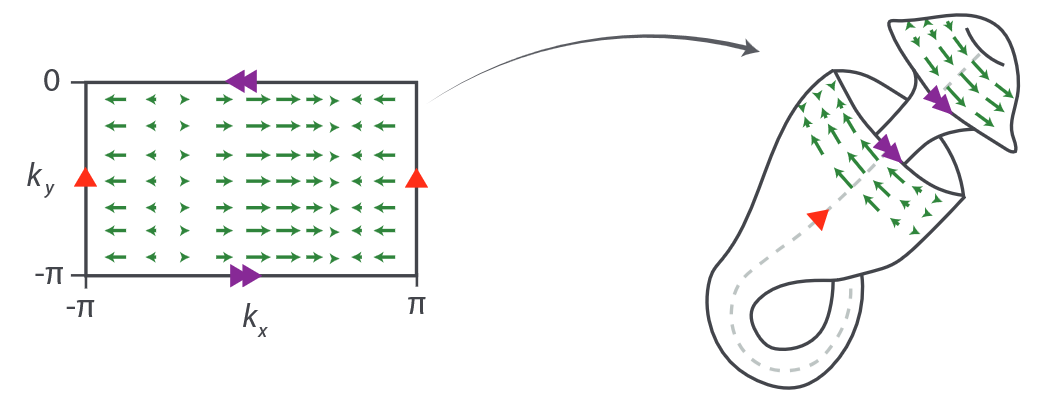
\includegraphics[width=.8\linewidth]{Images/Klein-discontinuity}
	\caption{Figure~from the supplement to Ref.~\cite{Fonseca-Vaidya_nonorientable}. The $k_x$ component of an example $\h(\k)$ is mapped onto a $K^2$ slice of the fundamental domain and then ``bent into shape'' to demonstrate discontinuity.
	}
	\label{fig:Klein-discontinuity}
\end{figure}
However, this mischaracterises the situation somewhat; in reality, $\h(\k)$ cannot be considered a well defined tangent vector field to $\KS$ to begin with. This is illustrated in Figure~\ref{fig:BZ_vectors}: two vectors which point away from each other in the fundamental domain may instead point towards each other after applying the glide symmetry.
\begin{figure}[htb!]
	\centering
	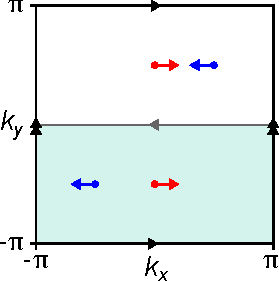
\includegraphics[width=.3\linewidth]{Images/BZ_vectors}
	\caption{Example values of $\h(\k)$, interpreted as a vector field on the glide symmetric Brillouin torus. Similar colours indicate that the points are related by glide symmetry. Between two such symmetry related points $\k$ and $\k'$, the relation $\h(\k)=\h(\k')$ implies that the direction of the vector is not reversed by the glide reflection. As a result, the vector field behaves differently between the two halves of $\T^3$, and so it is ill defined as a vector field on $\KS$.}
	\label{fig:BZ_vectors}
\end{figure}
As such, $\h$ should be thought of as a more abstract map $\KS\to\R^3$ rather than a tangent vector field. To be precise, $\h$ is a section of the trivial $\R^3$-bundle over $\KS$, not of its tangent bundle.\footnote{
	In the usual case of the torus, these descriptions are equivalent: $\T^3$ is parallelisable, i.e.\ $T\T^3\cong \T^3\times\R^3$. This is what allows Poincaré--Hopf to apply naturally.}
The resulting mod 2 charge cancellation is not necessarily a sign that Poincaré--Hopf has failed, but rather that we are operating outside its realm of applicability. In fact, instead of rendering the theorem broken in some way, it may be more constructive to reason the other way around. The argument goes as follows: Poincaré--Hopf usually holds because one can always locally induce a canonical orientation on the tangent bundle from an orientation on the manifold itself. However, in the case of a map $\KS\to\R^3$, one has an orientable $\R^3$-bundle over a non-orientable base manifold. This means that the orientation of the bundle becomes fundamentally disconnected from that of the manifold, and a relative orientation between the two must be chosen arbitrarily and---since the base manifold does not admit a global orientation---locally. The mod 2 charge cancellation then tells us how Poincaré--Hopf needs to be modified to accommodate this arbitrary orientation: in some sense it gives rise to a ``generalised'' or ``modified'' Poincaré--Hopf theorem. Note that choosing between different fundamental domains on the torus (in the way outlined in Figure~\ref{fig:BZ_param}) is precisely a way of inducing such a relative orientation between $\KS$ and its $\R^3$-bundle; we will see this idea play out in more detail once we derive the mod 2 charge cancellation from more fundamental cohomology arguments.

It is worth emphasizing that this modification of Poincaré--Hopf is a general feature of non-orientable manifolds, not one that is specific to the model Hamiltonian. Smooth tangent vector fields can in fact be defined on $\KS$, but a Hamiltonian cannot be associated to them in a canonical way. Such a construction usually requires using gamma matrices that ``twist along'' with the tangent bundle of the manifold instead of the regular vector of Pauli matrices, but these gamma matrices cannot be defined consistently on a non-orientable manifold.\footnote{
	The proper construction is that of a Clifford algebra bundle over the tangent bundle, see Section 4.2 of Ref.~\cite{Mathai_math-review}. This construction relies on the existence of a so-called \emph{spin$^c$ structure} (essentially a basis of spinors) on the base manifold, but non-orientable manifolds do not admit such a structure on their tangent bundle.}
As a result, the notion of a tangent vector field loses some of its utility in studying the topological properties of a non-orientable system. Instead, any topological analysis must be performed in terms of more fundamental algebraic topology tools, such as the homology and cohomology relied on in this work.

A final point that merits clarification is the inclusion of a second glide symmetry. The supplement to Ref.~\cite{Fonseca-Vaidya_nonorientable} discusses imposing Equation~\eqref{eq:3D_glide} together with a similar symmetry along the glide plane $k_y = 0$:
\begin{equation}
	H(k_x, k_y, k_z) = H(k_x + \pi, -k_y, k_z).
\end{equation}
It is claimed that this double symmetry subdivides the 3-torus into four copies of a different non-orientable manifold $\RP^2\times S^1$. Here $\RP^2$ is the real projective plane, i.e.\ the space of all lines through the origin in $\R^3$; it can be obtained by identifying all antipodal points on a 2-sphere. In this case, $\RP^2\times S^1$ is obtained by imposing anti-periodic boundary conditions in both the $k_x$ and $k_y$ directions on a quarter of the Brillouin torus. However, this direct identification with $\RP^2\times S^1$ cannot be made as straightforwardly as in the case of a single glide symmetry. As discussed in our review of Refs.~\cite{HZY_RP2} and \cite{WangZhang_acoustic-Klein-2D} in Section~\ref{sec:review}, the combination of two perpendicular glide symmetries in two dimensions does not have a free action, leading to the fixed points shown in Figure~\ref{fig:Pgg-fixed-points}.

The situation is analogous in three dimensions: the four lines at the momenta $\k = (\pm\pi/2,\pm\pi/2,k_z)$ are fixed under application of both glide symmetries at once. As a result, a Weyl point existing on one of these lines must have an even chirality, and it only has one symmetric partner in the 3-torus rather than the three one would expect from four identical copies of $\RP^2\times S^1$.\footnote{
	One can also argue that this must be the case topologically: if a manifold $M$ has an $n$-sheeted cover $\tilde{M}$, then the Euler characteristics of both spaces must be related by $\chi(\tilde{M}) = n\chi(M)$. Reducing the system down to two dimensions, we find $\chi(\T^2) = 0$ and $\chi(\RP^2) = 1$, so that the former cannot cover the latter. Instead, the only possible covering space for $\RP^2$ is the double cover $S^2\to\RP^2$, since $\chi(S^2) = 2$. Technically speaking, this means the fundamental domain needs to be described as an \emph{orbifold} rather than a manifold, i.e.\ a space that encodes data about orbits of a group action. For example, the Euler characteristic of $\RP^2$ is zero as an orbifold.}
Such Weyl points are physically fine-tuned and are expected to split into pairs under perturbations. Nevertheless, additional symmetries may exist which force Weyl points to exist on these lines, in which case the exceptional behaviour becomes key to the description \cite{Leonhardt_symmetry-enforced}. Moreover, the reduction to a fundamental domain is predicated on a free group action in the main text of Ref.~\cite{Fonseca-Vaidya_nonorientable}. As such, analysis of a purely $\RP^2\times S^1$ Brillouin zone cannot a priori be expected to provide the correct topological classification for this double glide symmetry. Indeed, similar to the case of time reversal in Section~\ref{sec:T-WSMs}, a proper classification scheme should involve equivariant cohomology on the torus, bearing in mind the topological role of the high-symmetry points.
 \footnote{The mathematical description may be further complicated by the fact that the high-symmetry points are fixed only by a proper subgroup of the symmetry group. Beyond equivariant cohomology, the natural setting may be to treat $\RP^2\times S^1$ as an \emph{orbifold} rather than a manifold, i.e.\ a space that encodes data about orbits of a group action. For example, the Euler characteristic of $\RP^2$ is zero as an orbifold. These spaces can be analysed using the highly specialised tool of \emph{orbifold cohomology}; see for example Ref.~\cite{Adem_orbifold-cohomology} for an application to crystallographic symmetries.}
This becomes manifestly clear from the existence of a topological invariant at these high-symmetry points \cite{HZY_RP2,WangZhang_acoustic-Klein-2D}. This full analysis is somewhat beyond the scope of the present text, and in what follows we will restrict our attention to the case of a single glide symmetry.

\subsection{Classification scheme}\label{sec:formalism}

There are two main conceptual challenges that present themselves in attempting to apply consistent cohomology and homology frameworks to non-orientable systems, and in particular in developing a physical intuition for them. First of all, the analogy between second cohomology classes and differential two-forms such as the Berry curvature $\Fc$ breaks down in this case, and a statement like Equation~\eqref{eq:2nd-cohom-t3} can no longer be taken to hold directly. This is because differential forms like $\Fc$ cannot be integrated over non-orientable manifolds, and the associated (de Rham) cohomology group is actually real-valued---as discussed in Section~\ref{sec:cohomology}, it cannot readily encode the $\Z_2$ invariants induced by changes in orientation. As an example, suppose we are trying to find an invariant for the 2D Klein bottle insulator obeying Equation~\eqref{eq:2D_glide}. Integrating a Berry curvature on $K^2$ directly is not well defined, while integrating over the entire Brillouin torus always yields zero: the integration is over two oppositely oriented areas. The correct $\Z_2$ invariant can be interpreted as integration with different signs on both halves of the torus, bearing in mind that the result is only gauge invariant mod 2. In order to capture this behaviour generally, we need to move to the richer but more abstract integer-valued cohomology laid out in Section~\ref{sec:homology-cohomology}.

The second obstacle is that Poincaré duality is altered in this context. In Section \ref{sec:semimetal-topology}, this form of duality was used to identify the familiar cohomology invariants with homology invariants, in the form of non-trivial oriented loops and Dirac strings. In a non-orientable system, this identification cannot be made directly; in this case, either the homology or the cohomology must be twisted by the introduction of a local coefficient system $\ext{\Z}$ \cite{Whitehead_Homotopy,Hatcher_algebraic-topology}; this is the same notion of local coefficients discussed in Section~\ref{sec:T-WSMs}. Such a coefficient system compensates for the twist in orientation by tracking sign changes across the manifold.\footnote{
	Technically speaking, we are specifically describing local coefficients \emph{in the orientation sheaf}, i.e.\ twisted along the local orientation of the manifold. In general, the coefficients can be twisted along any $\Z$-bundle over the manifold, and in particular the trivial bundle gives normal coefficients in $\Z$.} 
Introducing local coefficients on an $n$-manifold $M$ gives rise to the twisted homology and cohomology groups $H_k(M;\ext{\Z})$ and $H^k(M;\ext{\Z})$. Poincaré duality then takes the following forms \parencite[Theorem 3H.6]{Hatcher_algebraic-topology}:
\begin{align}
	H_k(M;\ext{\Z}) &\cong H^{n-k}(M), \label{eq:twisted-hom-duality}\\
	H^k(M;\ext{\Z}) &\cong H_{n-k}(M). \label{eq:twisted-cohom-duality}
\end{align}
That is, twisting either one of the homology or cohomology restores Poincaré duality; if the homology is twisted, ordinary cohomology must be used and vice versa. When $M$ is orientable, the local coefficients become trivial and the original form of Poincaré duality is recovered from both relations.\footnote{
	The twist in the orientation sheaf is necessary to have Poincaré duality in the non-orientable case, but technically it need not be the only twist in the coefficients; additional twists may be added to both the homology and cohomology simultaneously without breaking the duality again \parencite[\S~5.2.2.]{DavisKirk_algebraic-topology}, and this is also true in the orientable case. This appears to be superfluous in this case, but it may become useful when dealing with non-trivial projections onto the surface.}

Given the fact that Poincaré duality can be restored by twisting either the homology or the cohomology group, the correct classification of a non-orientable physical system hinges on this choice of twist. Fortunately, there is a straightforward way to decide between the two in the case of a Weyl semimetal with an orientation-reversing $\Z_2$ symmetry. In this situation, Poincaré duality is necessary in order to relate the chirality of Weyl points (which are cohomology invariants) to the orientation of their corresponding Dirac strings (which are the dual homology invariants). Under the orientation-reversing symmetry, Poincaré duality breaking manifests itself in the fact that the Weyl point chiralities are naturally reversed, while the orientation of Dirac strings is unchanged. This is illustrated schematically in Figure~\ref{fig:local_coefficients}.
\begin{figure}[htb!]
	\centering
	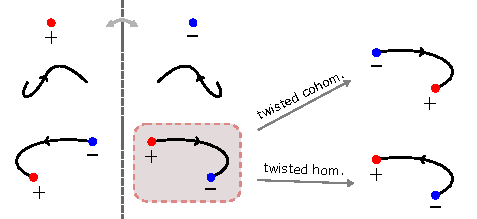
\includegraphics[width=.9\linewidth]{Images/local_coefficients}
	\caption{On the top left, the action of an orientation-reversing symmetry (represented by the dashed mirror axis) is shown on a Weyl point [of which the chirality is an invariant in $H^2(M\setminus W)$] and a Dirac string  [representing an invariant in $H_1(M,W)$]. The Weyl point has its chirality reversed, since the Chern number is a pseudoscalar. On the other hand, the Dirac string is mirrored but maintains its internal orientation (i.e.\ its image is also oriented away from the ``hook'' at the end). As a result, when the symmetry acts on a set of two Weyl points connected by a Dirac string, the resulting structure (shown in the shaded area) has a Dirac string of which the orientation is inconsistent with the chirality of the Weyl points, pointing from positive to negative---this is a result of Poincaré duality breaking. This problem can be resolved in one of two ways: either the cohomology is twisted into $H^2(M\setminus W;\ext{\Z})$ to undo the chirality reversal of the Weyl points, or the homology is twisted into $H_1(M,W;\ext{\Z})$ to reverse the Dirac string's orientation. Poincaré duality is restored in both cases; the correct approach depends on the physical setup.}
	\label{fig:local_coefficients}
\end{figure}
The decision of which group must be twisted can thus be made by noting how the chirality of Weyl points (outside of high-symmetry points) relates to that of their symmetric partners in the full Brillouin torus. To be precise, the presence of same-chirality pairs indicates that the (cohomological) Chern number is not reversed as expected, and the cohomology must be twisted. Meanwhile, pairs with opposite chiralities indicate that the cohomology behaves naturally, and the homology (i.e.\ the Dirac string orientations) must be twisted to follow suit.

There is a natural physical constraint on this relative chirality between symmetry-related Weyl points: if the orientation-reversing symmetry is unitary, then Weyl points have symmetric partners of opposite chiralities. This can be seen as follows: in the case of a unitary symmetry relating $\k\leftrightarrow\k'$, the Hamiltonian obeys
\begin{equation*}
	U\Hc(\k)U^{-1} = \Hc(\k').
\end{equation*}
If $\ket{\psi(\k)}$ is an eigenstate of $\Hc(\k)$, it follows that $\ket{\psi(\k')}:=U\ket{\psi(\k)}$ is an eigenstate of $\Hc(\k')$, and so the Berry connection transforms as
\begin{DispWithArrows*}[fleqn, displaystyle]
	\Ac(\k) &= i\braket{\psi(\k) | \dee_{\k}\psi(\k)}\cdot\dd{\k} \\
		&= i\braket{\psi(\k') | UU^{-1} | \dee_{\k}\psi(\k')}\cdot\dd{\k} \Arrow{$UU^{-1}=\Id$, $\dee_{\k}f\cdot\dd{\k} = \dee_{\k'}f\cdot\dd{\k'}$} \\
		&= i\braket{\psi(\k') | \dee_{\k'}\psi(\k')}\cdot\dd{\k'} \\
		&= \Ac(\k').
\end{DispWithArrows*}
Since the Berry connection one-form is left invariant, so is the Berry curvature two-form. A final minus sign is then induced by the change of orientation when integrating this two-form, so that the Chern number (Weyl point chirality) changes sign under unitary orientation-reversing symmetries. This is exactly what is implied when the Chern number is called a pseudoscalar. Referring back to Figure~\ref{fig:local_coefficients}, we conclude that twisted homology (and its dual ordinary cohomology) must be used to obtain the correct invariants under unitary symmetries.

%On the other hand, under an anti-unitary symmetry the Hamiltonian transforms as \red{[for $\TRS^2=-1$]}
%\begin{equation*}
%	U\Hc(\k)U\herm = \Hc^*(\k'),
%\end{equation*}
%and its eigenstates obey $\bra{\psi(\k')} = U\ket{\psi(\k)}$. The unitary matrix $U$ drops out of the Berry connection as before, and we are left with
%\begin{align*}
%	\Ac(\k) &= i\braket{\psi(\k) | \dee_{\k}\psi(\k)}\cdot\dd{\k} \\
%		&= i\braket{\dee_{\k'}\psi(\k') | \psi(\k')}\cdot\dd{\k'} \\
%		&= -\left(i\braket{\psi(\k') | \dee_{\k'}\psi(\k')}\right)^*\cdot\dd{\k'} \\
%		&= -\Ac^*(\k') = -\Ac(\k'),
%\end{align*}
%where the last equality holds because $\Ac$ is a real-valued one-form. It follows that the Berry curvature and its associated Chern numbers pick up an additional minus sign, which cancels out the orientation reversal. As a result, Weyl points have the same sign as their symmetric partners, and the correct description is given by twisted cohomology and ordinary homology.

The anti-unitary case is more difficult to pin down: the relative chirality of symmetric pairs of Weyl points may be either equal or opposite under anti-unitary symmetry \cite{Abdulla_chiral-WSM}. This is where the line of reasoning set out in Figure~\ref{fig:local_coefficients} is most useful. As an example, we apply this argument to the time-reversal invariant Weyl semimetal from Section~\ref{sec:T-WSMs}. This system is not usually thought of in terms of non-orientability, but the time reversal symmetry acts in an orientation-reversing way: an odd number (i.e.\ all three) of momentum directions are inverted, leading to a change of parity. Figure~\ref{subfig:TRS_orientation} illustrates that the effective Brillouin zone\footnote{
	Recall from Section~\ref{sec:T-WSMs} that the effective Brillouin zone indicates the quotient $\T^3 / \Z_2$ of the Brillouin torus by the symmetry group. In this case, the presence of high-symmetry points prevents this region from being a proper Brillouin zone, which is why we do not call it a fundamental domain.}
is indeed non-orientable.
\begin{figure}[htb!]
	\centering
	\subcaptionbox{\label{subfig:TRS_orientation}}{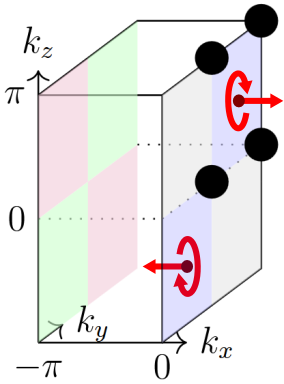
\includegraphics[width=.35\textwidth]{Images/TRS_EBZ_orientation}}
	\hfil
	\subcaptionbox{\label{subfig:TRS_Kramers}}{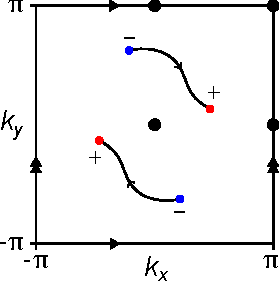
\includegraphics[width=.45\textwidth]{Images/Kramers_pairs}}
	\caption{(a) Figure~adapted from Ref.~\cite{Thiang_equivariant}. The effective Brillouin zone under time reversal symmetry is half of $\T^3$, with additional identifications of the coloured areas as $k\sim -k$. The resulting space is non-orientable: a ``test particle'' with a given helicity (obeying a left hand rule) is shown travelling out through the top right of the $k_x = 0$ boundary, and reappearing at its bottom left with the opposite helicity (obeying a right hand rule).
		(b) Top view of the Brillouin torus for a time-reversal invariant Weyl semimetal. The two (red) positively charged Weyl points are interrelated by the $\k\leftrightarrow-\k$ symmetry, as are the (blue) negatively charged points. These pairs of same-chirality points indicate a twist in the cohomology. On the other hand, the orientation of Dirac strings respects the symmetry, indicating ordinary (``untwisted'') homology.}
	\label{fig:TRS_twist}
\end{figure}
As discussed before, the pairs of Weyl points at opposite momenta (related by $\k\leftrightarrow -\k$) always have the same chirality in this system; see Figure~\ref{subfig:TRS_Kramers}.  %As discussed before, such systems feature Kramers pairs of Weyl points at opposite momenta related by $\k\leftrightarrow -\k$, both of which always have the same chirality; see Figure~\ref{subfig:TRS_Kramers}.
Again, these same-chirality pairs are an indication that the Chern numbers of Weyl points do not transform as expected, and so the cohomology must be twisted. It follows that the homology should be left untwisted; this can also be seen directly from the Dirac strings in Figure~\ref{subfig:TRS_Kramers}, whose orientation is directly related by the symmetry (i.e. the arrows run in relative directions respecting $\k\leftrightarrow-\k$). This description in terms of twisted cohomology and ordinary homology agrees exactly with the one given in Section \ref{sec:T-WSMs}, which was derived from more abstract vector bundle classification arguments in Ref.~\cite{Thiang_equivariant}. In this particular case, direct calculation of the (co)homology groups on the effective Brillouin zone is complicated by the existence of high-symmetry points (i.e.\ the action of the symmetry is not free), which is why the authors of Ref.~\cite{Thiang_equivariant} use equivariant (co)homology on the full torus.

Returning to the case of a momentum-space glide symmetry, we can infer from Figure~\ref{subfig:BZ_basic} that the situation is different here. The unitary nature of the symmetry [which is explicitly seen in Equation~\eqref{eq:3D_glide}] ensures that every Weyl point in the fundamental domain is related by symmetry to an oppositely charged point in the other half of the torus, while the orientation of Dirac strings is reversed under the symmetry. It follows that the classification of topological phases should rely on twisted \emph{homology}, and equivalently, ordinary cohomology. Since there are no high-symmetry points in this case, there is no need to compute equivariant (co)homology groups, and we may instead rely on ordinary cohomology and twisted homology on the fundamental domain $\KS$.\footnote{\label{ft:eq_cohom}
	Formally speaking, equivariant cohomology of a space $M$ with a free action of the group $G$ is equivalent to ordinary cohomology on the quotient space $M/G$ \parencite[Corollary 9.6]{Tu_equivariant}.}

The choice of ordinary cohomology can be corroborated in two important ways. Firstly, the use of ordinary second cohomology classes indicates that we are classifying complex line bundles over the fundamental domain. An important insight from K-theory tells us that this is equivalent to classifying equivariant line bundles over the full torus \parencite[Proposition 2.1]{Segal_K-theory}.\footnote{
	This is related to footnote \ref{ft:eq_cohom} in the sense that K-theory is a \emph{generalised cohomology} theory.}
That is, we are classifying states that respect the symmetry directly. Secondly, the $\Z_2$ invariant found in Ref.~\cite{Fonseca-Vaidya_nonorientable} on $K^2$-like slices of constant $k_z$ is recovered using ordinary cohomology, related to the fact that $H^2(K^2)\cong\Z_2$. Twisted cohomology would give a $H^2(K^2;\ext{\Z})\cong\Z$ invariant on these slices.

All in all, we find that the correct classification of semimetal phases in this system is given by the following Mayer--Vietoris exact sequence of cohomology groups on $M := \KS$:
\begin{equation}\label{eq:MV-nonorientable}
	0\ \to\ \underbrace{H^2(M)}_{\mathclap{\text{Insulator}}}\ \to\ \underbrace{H^2\big(M\setminus W\big)}_{\mathclap{\text{Semimetal}}}\ \to\ \bigoplus_{w\in W} H^2(S_w^2)\ \overset{\Sigma}{\to}\ H^3(M)\ \to\ 0,
\end{equation}
where as before, $W$ is the set of Weyl points on $M$ and $S_w^2$ is a small 2-sphere surrounding the Weyl point $w\in W$. Equivalently, the classification may be given in terms of the following dual \emph{twisted} homology sequence:
\begin{equation}\label{eq:homology-sequence-nonorientable}
	0\ \to\ \underbrace{H_1(M;\ext{\Z})}_{\mathclap{\text{Twisted Dirac loops}}}\ \to\ \underbrace{H_1(M, W;\ext{\Z})}_{\mathclap{\text{Twisted Dirac strings}}}\ \overset{\partial}{\to}\ H_0(W;\ext{\Z})\ \overset{\Sigma}{\to}\ H_0(M;\ext{\Z})\ \to\ 0,
\end{equation}
where we refer to the Dirac loops and Dirac strings as twisted to emphasise the non-trivial action of the symmetry on their orientation. The concept of a twisted Dirac string on $\KS$ can be difficult to intuit, leading to Dirac strings that appear to change orientation at orientation-reversing boundaries of the fundamental domain in a setup like Figure~\ref{subfig:BZ_right}. As such, they are more readily understood as equivariant (i.e.\ symmetry-related) pairs of Dirac strings on the full torus $\T^3$, of which the orientation is reversed under the symmetry.

In what follows, we will provide explicit computations of these sequences and discuss the associated invariants.


\subsection{Computation of invariants on \texorpdfstring{$\KS$}{K²×S¹}}\label{sec:invariants}

The use of ordinary cohomology groups in the Mayer--Vietoris sequence \eqref{eq:MV-nonorientable} means that calculations are relatively straightforward, and standard techniques such as cellular cohomology can be applied. \red{[Given enough time, I can include a small Appendix B containing an example cellular cohomology calculation.]} %TODO appendix or ref.
Using these methods, we calculate the sequence to be
\begin{equation}\label{eq:explicit-sequence-nonorientable}
	0\to \Z\oplus\Z_2 \overset{\alpha}{\to} \Z\oplus\Z_2\oplus\Z^k \overset{\beta}{\to} \Z^k \overset{\Sigma}{\to} \Z_2 \to 0,
\end{equation}
where $k = |W|$ is the number of Weyl points. Given that the twisted homology sequence \eqref{eq:homology-sequence-nonorientable} is related to the Mayer--Vietoris sequence by Poincaré duality, it features the exact same groups in the same order; the difference is only in the interpretation. 

For comparison, we recall here the semimetal Mayer--Vietoris sequence on $\T^3$ from Section \ref{sec:Mayer-Vietoris}:
\begin{equation}\label{eq:semimetal-MV-explicit-again}
	0 \to \Z^3 \to \Z^3\oplus\Z^{k-1} \overset{\beta}{\to} \Z^k \overset{\Sigma}{\to} \Z \to 0.
\end{equation}
Some relevant differences between these two sequences are highlighted below.

\subsubsection{Insulating phases}

The first difference between the Mayer--Vietoris sequences on $\T^3$ and $\KS$ lies in the insulating topology of the system, in the absence of any Weyl points. Whereas the 3D Chern insulator on the plain torus features a Chern vector in $H^2(\T^3)\cong\Z^3$, this group is reduced to $H^2(\KS)\cong\Z\oplus\Z_2$ under the action of the glide symmetry. As a result, the $\KS$ insulator is not classified by three Chern numbers $C_{x,y,z}\in\Z$, but by a $\Z$ invariant $\nu_x$ and a $\Z_2$ invariant $\nu_z$---the reasoning behind our choice of symbols will become apparent shortly.

The reduction to two invariants can be most readily understood from the twisted homology point of view. On $\T^3$, the three generators of $H_1(\T^3)\cong\Z^3$ are represented by oriented Dirac loops $\ell_{x,y,z}$ that wind around the 3-torus once in each respective coordinate direction. Under glide symmetry, each of these loops obtains a symmetric partner $\ell_{x,y,z}'$ with a reversed internal orientation---this is due to the twist in the homology. Taken together with the original loop, $\ell_{x,y,z} + \ell_{x,y,z}'$ is equivalent to a twisted Dirac loop $\tilde{\ell}_{x,y,z}$ on $\KS$, representing an invariant in $H_1(\KS;\ext{\Z})$. The reduction to $\Z\oplus\Z_2$ is then caused by specific degeneracies in these twisted Dirac strings: $\tilde{\ell}_x$ generates the full $\Z$ invariant $\nu_x$, $\tilde{\ell}_y$ turns out to be trivial, and $\tilde{\ell}_z$ generates the $\Z_2$ invariant $\nu_z$. This is illustrated in more detail in Figure \ref{fig:K2S1_invariants}.
\begin{figure}[htb!]
	\centering
	\subcaptionbox{$[\tilde{\ell}_x]$\label{subfig:Z_invariant}} {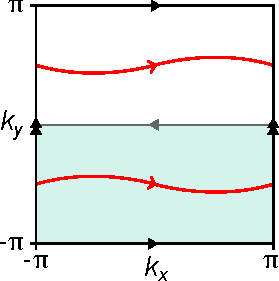
\includegraphics[width=.3\textwidth]{Images/Z_invariant}}
	\hfil
	\subcaptionbox{$[\tilde{\ell}_y] = 0$\label{subfig:0_invariant}} {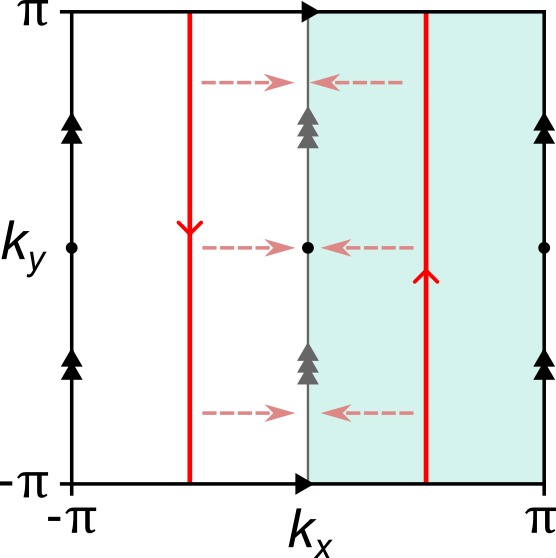
\includegraphics[width=.3\textwidth]{Images/0_invariant}}
	\hfil
	\subcaptionbox{$[\tilde{\ell}_z] = [-\tilde{\ell}_z]$\label{subfig:Z2_invariant}} {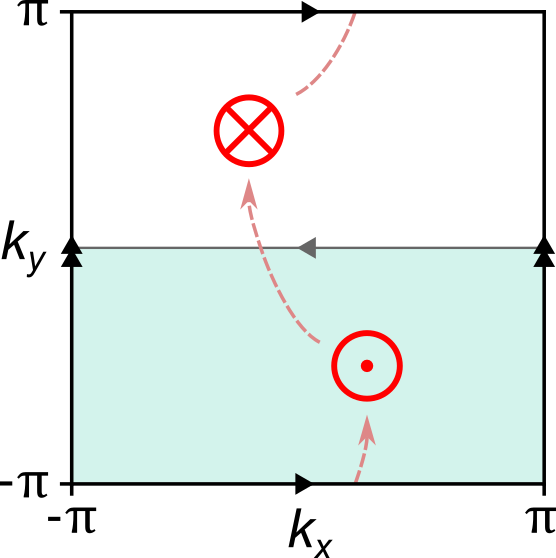
\includegraphics[width=.3\textwidth]{Images/Z2_invariant}}
	\caption{Top view of $\T^3$. Each graphic shows one of the three basic Dirac loops $\ell_{x,y,z}$ [representing the generators of $H_1(\T^3)$] sitting inside a fundamental domain (shaded teal). Each loop is doubled by the action of the symmetry, into what can be considered a twisted Dirac loop $\tilde{\ell}_{x,y,z}$ [representing an invariant in $H_1(\KS;\ext{\Z})$] shown in red. (a) In the case of $\ell_x$, the orientation reversal cancels out the $k_x \mapsto -k_x$ parity change from the glide symmetry, and the resulting twisted Dirac string $\tilde{\ell}_x$ has a consistent orientation. It follows that the associated invariant $\nu_x\in\Z$ induces an even Chern number $C_x = 2\nu_x\in 2\Z$ on the full torus.
		(b) The alternative fundamental domain from Figure \ref{subfig:BZ_right} paints a clearer picture for $\ell_y$. The loop is mirrored along the glide plane $k_x=0$ and has its orientation reversed. The resulting twisted Dirac string $\tilde{\ell}_y$ is trivial: as indicated by the dashed arrows, the two copies can be moved together while maintaining glide symmetry, and they cancel out when they meet on the glide plane. As a result, there is no invariant $\nu_y$.
		(c) The Dirac loop $\ell_z$ running in the positive $z$ direction (``out of the page'') in the fundamental domain is doubled to a second loop running in the negative $z$ direction (``into the page''). In this case, the two loops cannot be brought together while respecting the symmetry, but they can be interchanged by moving them along the dashed arrows. It follows that the resulting twisted Dirac string $\tilde{\ell}_z$ is equivalent to its own inverse $-\tilde{\ell}_z$, meaning it generates a $\Z_2$ invariant $\nu_z$.}
	\label{fig:K2S1_invariants}
\end{figure}

The invariant $\nu_z\in\Z_2$ corresponds precisely to the $\Z_2$ invariant on $K^2$ slices described in Ref.~\cite{Fonseca-Vaidya_nonorientable}, and stems from the 2D Klein bottle insulator in Ref.~\cite{CYZ_Klein-gauge}. It may be calculated on any $K^2$ slice using Equations~\eqref{eq:z2-inv1} and \eqref{eq:z2-inv2}. 

The $\Z$ invariant $\nu_x$ appears to be novel; as discussed under Figure~\ref{subfig:Z_invariant}, it manifests as an even Chern number $C_x = 2\nu_x\in 2\Z$ on the full Brillouin torus, relating to the fact that the torus contains two copies of $\KS$. This suggests one way of calculating this invariant in practice: it may be obtained from $\T^3$ as
\begin{equation}\label{eq:z-invariant1}
	\nu_x = \frac{1}{2}C_x = \frac{1}{4\pi}\int_{\T_{yz}^2}\!\Fc,
\end{equation}
where $\T_{yz}^2$ is any slice of $\T^3$ running in the $yz$-direction. This calculation does not generally respect the glide symmetry, since such a $\T_{yz}^2$ is not invariant outside of the glide planes at $k_x=0$ and $k_x = \pm\pi$. Still, it results in the correct invariant in the insulating case: by regular Poincaré duality on the full torus, the integral over $\T_{yz}^2$ counts the number of $\ell_x$-like Dirac loops, and the generator $\tilde{\ell}_x$ features precisely two such loops on the torus.\footnote{
	A Dirac loop may in principle also contain $y$ and $z$ components, but these do not affect this integral. From a homology perspective, such loops may be decomposed into their basic $\ell_{x,y,z}$ components because the first homology group is Abelian.}
We will return to the case with Weyl points when we study the full group of semimetal invariants.

\subsubsection{Mod 2 charge cancellation}

A second feature that stands out is the appearance of a $\Z_2$ group on the far right side of the exact sequence in Equation~\eqref{eq:explicit-sequence-nonorientable}. It is worth mentioning that this is a general feature of ordinary cohomology on non-orientable manifolds: the rightmost group is the top cohomology group of the fundamental Brillouin zone, and any non-orientable $n$-manifold $M$ has $H^n(M)\cong\Z_2$.

Recall from Section \ref{sec:Mayer-Vietoris} that the map $\Sigma$ in Equation~\eqref{eq:semimetal-MV-explicit-again} can be interpreted as a sum over all Weyl point charges on $\T^3$. The Nielsen--Ninomiya charge cancellation theorem on the torus then arises from the fact that $\Sigma\circ\beta = 0$; that is, a semimetal structure $a\in\Z^3\oplus\Z^{k-1}$ must always feature a charge configuration $\beta(a)\in\Z^k$ such that the charges sum to $\Sigma(\beta(a)) = 0 \in \Z$.

The situation is somewhat more subtle on $\KS$: the $\Z^k$ group $H^2\!\left(\bigcup_{i=1}^k S_{w_i}^2\right)$ and its dual $H_0(W;\ext{\Z})$ no longer have a direct interpretation in terms of Weyl point charges, since both the absolute and relative chiralities of these points are ill defined (see Figure~\ref{fig:BZ_param}). That is, the spheres $S_{w_i}$ no longer have a canonical orientation descending from the ambient manifold.\footnote{
	This is closely related to our observation in Section~\ref{sec:clarifications} that Poincaré--Hopf fails to apply because the trivial $\R^3$-bundle over $\KS$ does not have a canonical orientation with respect to its base manifold.}
Instead, $H^2\!\left(\bigcup_{i=1}^k S_{w_i}^2\right)$ must be interpreted as the group of charges $\chi_i$ \emph{given a choice of orientation} at each Weyl point $w_i$. This choice of orientation is exactly what is induced by choosing a specific fundamental domain: the changes of (absolute and relative) chirality in Figure~\ref{fig:BZ_param} correspond to a change of basis of this $\Z^k$. Nevertheless, the map $\Sigma$ can still be interpreted as a sum over these charges, precisely because it maps into $\Z_2$:\footnote{
	Indeed, the group $H^3(\KS)\cong\Z_2$ is closely linked to the orientation of $\KS$; in technical terms, we say that $\KS$ is $\Z_2$-orientable but not $\Z$-orientable \parencite[\S 3.3]{Hatcher_algebraic-topology}.}
to be exact, the map
\begin{equation}\label{eq:map-sigma}
	\Sigma: \Z^k\to\Z_2,\quad (\chi_1,\ldots,\chi_k) \mapsto \sum_{i=1}^{k}\chi_i \mod 2
\end{equation}
is invariant under change of orientation at each $w_i$ because
\begin{equation*}
	\chi_i \equiv -\chi_i \mod 2.
\end{equation*}
It follows that the tail end of the sequence \eqref{eq:explicit-sequence-nonorientable} can be interpreted unambiguously in terms of $\Z_2$ charge cancellation: regardless of the parametrisation of the fundamental domain, the charges belonging to a semimetal (i.e.\ mapped into $\Z^k$ by $\beta$) must sum to $0\in\Z_2$. This is the same charge cancellation condition presented in Equation~\eqref{eq:Z2-cancellation}.

Importantly, the exactness of Equation~\eqref{eq:explicit-sequence-nonorientable} also implies the converse statement by $\im(\beta) = \ker(\Sigma)$: for a given set of Weyl points $W\subset \KS$, any configuration of charges with an even total [i.e.\ an element of $\ker(\Sigma)$] must be realised in some set of semimetal invariants [i.e.\ be an element of $\im(\beta)$]. In the homology picture, this means there must exist configurations of twisted Dirac strings in $H_1\big(M, W;\ext{\Z}\big)$ realising any given set of charges adding to $0\in\Z_2$.

One must be careful in interpreting this mod 2 charge cancellation in terms of a potentially non-zero total chirality. The $\Z_2$ group in the Mayer--Vietoris sequence tells us that total charge is fundamentally a $\Z_2$ invariant, and the semimetal topology fixes it to zero. Given any particular parametrisation of the fundamental domain, there may appear to be a net non-zero chirality on the Brillouin zone $\KS$, but this is not a topological invariant: for example, in Figure~\ref{fig:BZ_param}, the net chirality of a single topological state may be found to be 0, 2 or -2 depending on the parametrisation. In other words, the total chirality is ill defined as an integer in $\Z$, while the \emph{parity} of the total charge is well defined and topologically invariant.

The appearance of non-zero total chirality is in close analogy to the concept of ghost fields in quantum field theory. There, apparent quantum fields may arise when fixing unphysical local gauge degrees of freedom. These ghost fields can usually be removed by a suitable change of gauge, and in any case they never appear in external physical observables. Similarly, the choice of orientation for a Weyl point on $\KS$ is an unphysical local degree of freedom, and one can usually choose these orientations (i.e.\ fix a fundamental domain) in a way that results in a total chirality of zero. In particular, this implies that one cannot readily assign physical meaning (e.g.\ in terms of an uncancelled chiral anomaly) to the net chirality appearing in a certain fundamental domain.

This can also be understood in field theory terms: as discussed in Section~\ref{sec:clarifications}, a Hamiltonian cannot be defined on $\KS$ in terms of the tangent vector field, since it lacks a spinor basis (i.e.\ choice of gamma/Pauli matrices). Instead, any effective field theory on $\KS$ must rely on a choice of coordinates, and will not be invariant under change of coordinates in general. In such a theory, a net chiral anomaly will not generally represent a physically observable phenomenon. In other words, while the Nielsen--Ninomiya theorem is altered mathematically on $\KS$, its core physical implications of chiral anomaly cancellation cannot necessarily be circumvented. In this respect, the description in terms of the full Brillouin torus $\T^3$ with a glide symmetry may be more useful phenomenologically, where Nielsen--Ninomiya is more straightforwardly preserved and each Weyl point has a canonical orientation.

\subsubsection{Semimetal invariants}

Finally, central to the sequence in Equation~\eqref{eq:explicit-sequence-nonorientable} is the group of semimetal invariants,
\begin{equation}\label{eq:semimetal-group-nonor}
	H^2(\KS\setminus W)\cong H_1(\KS, W; \ext{\Z})\cong \Z\oplus\Z_2\oplus\Z^k.
\end{equation}
Much like the $\Z^3\oplus\Z^{k-1}$ in the case of $\T^3$, this group does not admit a canonical basis of invariants. Rather, the exactness of Equation~\eqref{eq:explicit-sequence-nonorientable} around this group provides information about the structure of the different semimetallic phases. The argument is similar to that given for the torus at the end of Section~\ref{sec:Mayer-Vietoris}. In what follows, we make reference to the maps $\alpha$, $\beta$ and $\Sigma$ as defined in Equation~\eqref{eq:explicit-sequence-nonorientable}. Given a charge configuration $c\in\Z^k$ in the image of the map $\beta$ (i.e.\ any $c$ with an even total charge), the pre-image must obey
\begin{equation*}
	\beta^{-1}(c) \cong \beta^{-1}(0) =: \ker(\beta),
\end{equation*}
since $\beta$ is a homomorphism.\footnote{
	As before, this is a consequence of the first isomorphism theorem.}
By exactness, this can be calculated as $\ker(\beta)\cong\im(\alpha)\cong\Z\oplus\Z_2$.
That is, for each $c\in\im(\beta)$ there is a $\Z\oplus\Z_2$ of possible semimetal invariants (or equivalently, twisted Dirac string configurations) in its pre-image, differing from each other by the bulk invariants $\nu_x\in\Z$ and $\nu_z\in\Z_2$.

There is a subtle difference from the argument on the torus: on $\T^3$, $\Z$ charge cancellation ensures that the valid charge configurations exist in 
\begin{equation*}
	\im(\beta) = \ker(\Sigma) = \bigoplus_{w\in W} H^2(S_w^2) \Big/ H^3(\T^3) \cong \Z^k/\Z \cong \Z^{k-1},
\end{equation*}
explaining the $\Z^{k-1}$ summand in the semimetal group. This $\Z^{k-1}$ cannot be given a basis in terms of the $k$ different Weyl point charges on the semimetal, and it must be interpreted more abstractly as the set of valid charge configurations. On $\KS$, the $\Z_2$ charge cancellation implies that
\begin{equation*}
	\im(\beta)=\ker(\Sigma)\cong\Z^k/\Z_2\cong\Z^k,
\end{equation*}
and this is the $\Z^k$ which appears in the semimetal group in Equation~\eqref{eq:semimetal-group-nonor}. Just as on the torus, we should be careful not to interpret this $\Z^k$ directly in terms of the charges of the $k$ Weyl points. Even though it contains $k$ factors of $\Z$, not all possible combinations of charges are contained in this subgroup: after all, charge configurations with an odd total are not in the kernel of $\Sigma$. Instead, it should be considered an index 2 subgroup of the charge configurations, containing only those with an even total.

Physically, the $\Z^k$ summand in the semimetal group implies that a system with a single Weyl point ($k=1$) on $\KS$ may already feature semimetal topology, unlike the torus where a minimum of two points are needed. The single Weyl point must have even charge by $\Z_2$ charge cancellation; an example of such a system is featured in the supplement to Ref.~\cite{Fonseca-Vaidya_nonorientable} and reproduced in Figure~\ref{fig:double-points}.
\begin{figure}[htb!]
	\centering
	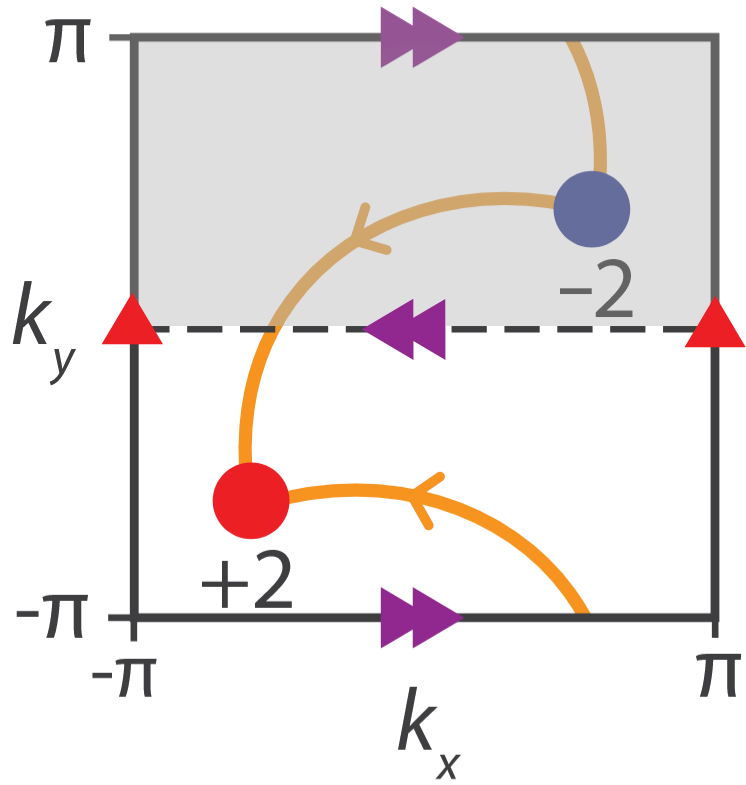
\includegraphics[width=.4\linewidth]{Images/double-points}
	\caption{Figure adapted from the supplement to Ref.~\cite{Fonseca-Vaidya_nonorientable}. Interpreted here as a top view of the Brillouin torus. The upper half lies outside of the fundamental domain and has been greyed out to emphasise that there is only one Weyl point on $\KS$. Both Dirac strings are oriented towards the positively charged point on the torus; from the perspective of the fundamental domain, there is a single twisted Dirac string, which reverses orientation as it crosses $k_y=0$ and is connected to the same Weyl point at both ends. Thinking more abstractly in terms of $\KS$, such an orientation-reversing boundary cannot be pointed out, and a consistent orientation cannot be assigned to this Dirac string---this is exactly what necessitates the use of twisted homology.}
	\label{fig:double-points}
\end{figure}

Finally, we have seen in Section~\ref{sec:Weyl-point-topology} that the Chern number on a 2D slice of $\T^3$ changes by $q\in\Z$ as the slice is passed over a Weyl point of charge $q$. We might expect this to be problematic in the non-orientable case, given that the fundamental Brillouin zone is (anti-)periodic and the total charge need not add up to zero. This is resolved in two different ways for the two invariants $\nu_x$ and $\nu_z$. The latter is saved by being a $\Z_2$ invariant, restoring the periodicity over an even total charge---as was also observed in Ref.~\cite{Fonseca-Vaidya_nonorientable}.

The $\Z$ invariant $\nu_x$ requires us to define the integration more carefully: as noted before, the integration in Equation~\eqref{eq:z-invariant1} does not respect the symmetry, and it may not yield the right invariant when Weyl points are introduced. This is illustrated in Figure~\ref{subfig:nu-x_wrong}.
\begin{figure}[htb!]
	\centering
	\subcaptionbox{\label{subfig:nu-x_wrong}} {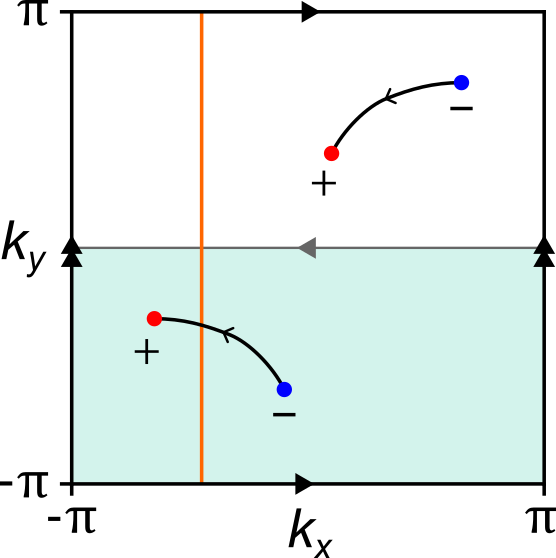
\includegraphics[width=.3\textwidth]{Images/nu-x_wrong}}
	\hfil
	\subcaptionbox{\label{subfig:nu-x_right}} {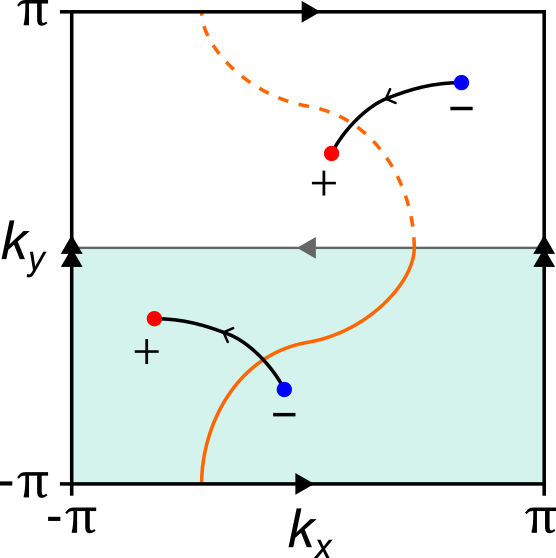
\includegraphics[width=.3\textwidth]{Images/nu-x_right}}
	\caption{(a) In the presence of Weyl points, a given $\T_{yz}^2$ (orange) may only intersect a single Dirac string, leading to a non-integer value of 1/2 from Equation~\eqref{eq:z-invariant1}. (b) Integration over an invariant surface always yields a well defined $\nu_x$ outside of Weyl points, since it intersects the twisted Dirac strings in a consistent manner. The dashed half of the surface is redundant, since both halves yield the same integral. The pictured setup yields $\nu_x=1$.}
	\label{fig:nu-x}
\end{figure}
Instead, it becomes necessary to integrate over a symmetry-invariant surface $S$ which is continuously deformable to a $\T_{yz}^2$, such as that shown in Figure~\ref{subfig:nu-x_right}. This is similar in spirit to the $\TRS$-invariant surfaces used to calculate invariants in the time-reversal symmetric case \cite{Thiang_equivariant}. In principle, only the half of the surface $S_{1/2}$ which intersects the fundamental domain at $k_y\leq 0$ needs to be integrated over; this half surface can be considered a compact surface subspace of $\KS$. The calculation then takes the form
\begin{equation}\label{eq:z-invariant2}
	\nu_x = \frac{1}{2\pi}\int_{S_{1/2}}\!\!\Fc.
\end{equation}
The question of periodicity is now resolved by the fact that the surface $S$ cannot be moved across the entire Brillouin torus without breaking the symmetry: any such surface can be deformed equivariantly into exactly one of the glide planes at $k_x=0$ and $k_x=\pm\pi$, but one cannot be deformed into the other. For example, if we start with $S$ at the $k_x=0$ plane and perturb a small section of $S$ continuously in the positive $x$ direction, then another section must be moved in the negative $x$ direction at the same time to maintain glide symmetry. By continuity, it follows that $S$ must still intersect $k_x=0$ somewhere.\footnote{
	The argument can be formalised using the mean-value theorem if we take the momenta to live in $\R^3$ rather than identifying equivalent momenta into a torus.}
As such, there is no deformation that can completely remove $S$ from the $k_x=0$ plane, and in particular it cannot be taken fully to the glide plane at $k_x=\pm\pi$. An analogous argument holds the other way around.\footnote{
	By the same logic, we can generally infer which of the two glide planes $S$ deforms to by studying these intersections: for example, the surface in Figure~\ref{subfig:nu-x_right} does not intersect the plane at $k_x=\pm\pi$, and so it must deform to $k_x=0$. In general, we can count the number of times $S$ intersects with $k_x=0$ in the range $-\pi<k_y\leq 0$ (at any $k_z$); an odd number of intersections [such as the single crossing in the fundamental domain in Figure~\ref{subfig:nu-x_right}] indicates that the surface deforms to $k_x=0$.}

As a final remark, we note that the only $\Z_2$ factor in the semimetal group in Equation~\eqref{eq:semimetal-group-nonor} stems directly from the underlying insulating topology; any Weyl points that are added only introduce additional $\Z$ factors. As such, it is the opinion of the author that no intrinsic $\Z_2$ charge should be assigned to Weyl points, as is done in Ref.~\cite{Fonseca-Vaidya_nonorientable}.\footnote{
	Explicit calculations are provided for this $\Z_2$ charge in Ref.~\cite{Fonseca-Vaidya_nonorientable}, but these rely on integration over $K^2$-like tubes spanning the fundamental domain in the $k_y$ direction. As a result, these invariants are an expression of the global topology of $\KS\setminus W$, not the local topology around a Weyl point.}
Instead, the $\Z_2$ invariant on gapped $K^2$-like slices should be taken to be directly influenced by the $\Z$ charge on Weyl points. To be precise, if such a slice with invariant $\nu_z$ is moved over a Weyl point of charge $C$ in the $k_z$ direction, the new $\Z_2$ invariant is
\begin{equation*}
	\nu_z' = \nu_z + C \mod 2,
\end{equation*}
requiring no $\Z_2$ charge on the Weyl point. This is also the position taken with respect to time-reversal invariant Weyl semimetals in Ref.~\cite{Thiang_equivariant}.


\subsection{Classification of \texorpdfstring{$K^2$}{K²} surface states}

We now turn our attention to the classification of surface states (i.e.\ Fermi arcs) on the two-dimensional surfaces of the $\KS$ system obeying the glide symmetry in Equation~\eqref{eq:3D_glide}. As mentioned in Section~\ref{sec:Weyl-point-topology}, Fermi arcs may be considered projections of the topological Dirac strings existing in the bulk. The same line of reasoning holds in this case: the twisted Dirac strings may be projected onto a surface Brillouin zone to obtain oriented Fermi arcs.

Of the three coordinate directions that we may project along, the $k_z$ direction is the most tractable, since there is no additional symmetry in this direction beyond the usual lattice translation. As such projecting along $k_z$ amounts to integrating out the periodic $S^1$ direction in $\KS$, to obtain a Klein bottle shaped $K^2$ surface Brillouin zone spanning the $k_x$ and $k_y$ directions. This is the surface that is discussed extensively and probed experimentally in Ref.~\cite{Fonseca-Vaidya_nonorientable}.

Because the projection $\pi_z$ along the $k_z$ direction loses no essential information about the symmetries of the system, it has a clear interpretation in terms of homology groups. Recall that, given a set of Weyl points $W\subset\KS$, a configuration of twisted Dirac strings $c$ defines a twisted relative homology class:
\begin{equation*}
	[c]\in H_1(\KS,W;\ext{\Z}).
\end{equation*}
The projection $\pi_z$ acts on $c$ to give a configuration of Fermi arcs $\pi_z(c)$. Taking into account the twist in orientation, $\pi_z(c)$ can be taken to represent a homology class:
\begin{equation*}
	[\pi_z(c)]\in H_1(K^2,W';\ext{\Z}),
\end{equation*}
where $W':=\pi_z(W)$ denotes the projection of the Weyl points on the surface. Formally, there is a surjective map
\begin{equation*}
	(\pi_z)_*: H_1(\KS,W;\ext{\Z}) \to H_1(K^2,W';\ext{\Z}),\quad [c] \mapsto [\pi_z(c)]
\end{equation*}
called the \emph{pushforward} of $\pi_z$ on homology classes. The surjectivity of this map ensures that all possible configurations of Fermi arcs in $H_1(K^2,W';\ext{\Z})$ are physically realisable, meaning this group provides a full classification of Fermi arcs on the $K^2$ surface.

The other groups in the twisted homology semimetal sequence in Equation~\eqref{eq:homology-sequence-nonorientable} may also be mapped by similar pushforwards of $\pi_z$, and in particular this operation preserves the nature of the maps featured in the sequence. This then gives rise to a similar exact sequence of twisted homology groups on the $K^2$ surface:
\begin{equation}
	0\ \to\ \underbrace{H_1(K^2;\ext{\Z})}_{\mathclap{\text{Twisted Fermi loops}}}\ \to\ \underbrace{H_1\big(K^2, W';\ext{\Z}\big)}_{\mathclap{\text{Twisted Fermi arcs}}}\ \overset{\partial}{\to}\ H_0(W';\ext{\Z})\ \to\ H_0(K^2;\ext{\Z})\ \to\ 0.
\end{equation}
We can then make use of twisted Poincaré duality in order to turn this into a more computable Mayer--Vietoris sequence of ordinary cohomology groups:\footnote{
	One needs to be a bit careful here in the sense that there is no longer a zero group to the left of the proper Mayer--Vietoris sequence, owing to the appearance of $H^0(S_{w'}^1)\cong\Z$ terms instead of the $H^1(S_w^2)=0$ in the bulk sequence. However, this does not change the interpretation of the sequence at all: the leftmost map into $H^1(K^2)$ is still trivial, since the circles $S_{w'}^1$ are contractible inside $K^2$.}
\begin{equation}\label{eq:K2-surface-cohomology}
	\cdots\ \overset{0}{\to}\ H^1(K^2)\ \to\ H^1\big(K^2\setminus W'\big)\ \to\ \bigoplus_{w'\in W'} H^1(S_{w'}^1)\ \to\ H^2(K^2)\ \to\ 0.
\end{equation}
Note that compared to the bulk sequence in Equation~\eqref{eq:MV-nonorientable}, this sequence classifies topological states in terms of first cohomology groups $H^1$ rather than second cohomology groups $H^2$. This is indicative of the fact that the chiralities of surface states are given by winding numbers of the Berry connection 1-form $\Ac$, rather than Chern numbers obtained from the Berry curvature 2-form $\Fc$.

Just as in the bulk, the Mayer--Vietoris sequence in Equation~\eqref{eq:K2-surface-cohomology} can be computed using standard tools such as cellular homology. %TODO appendix?
The resulting explicit sequence is as follows:
\begin{equation}\label{eq:K2-MV-explicit}
	\cdots \overset{0}{\to} \Z \to \Z\oplus\Z^k \to \Z^k \overset{\Sigma}{\to} \Z_2 \to 0.
\end{equation}
This sequence is very similar in nature and interpretation to the bulk sequence in Equation~\eqref{eq:explicit-sequence-nonorientable}. The only essential difference is that the insulating $\Z_2$ invariant $\nu_z$ has disappeared as a result of the projection in the $k_z$ direction.

In particular, this sequence features a similar mod 2 charge cancellation property to the one seen in the bulk, implying that the winding numbers of the Berry connection $\Ac$ around each projected Weyl node must add to a total of $0\in\Z_2$. Just as in the bulk, there is an important caveat regarding the physical interpretation of this: the sign of the winding number at a Weyl node $w$ depends on a choice of orientation for the circle $S_w^1$ that surrounds it. Just as in the bulk, this choice of orientation can be induced from a chosen fundamental domain, and this may lead to different relative chiralities between projected Weyl points.

As an example, the experimentally observed dispersion in Figure~\ref{fig:K2-experiment} depends on the choice of fundamental domain. That is, one can extend the $K^2$ surface Brillouin zone to the full $\T^2$ in this figure by including momenta with $0<k_2\leq\pi$, and then choose a different fundamental domain to change the relative chirality. This is illustrated in Figure~\ref{fig:K2-experiment-alt}.
\begin{figure}[htb!]
	\centering
	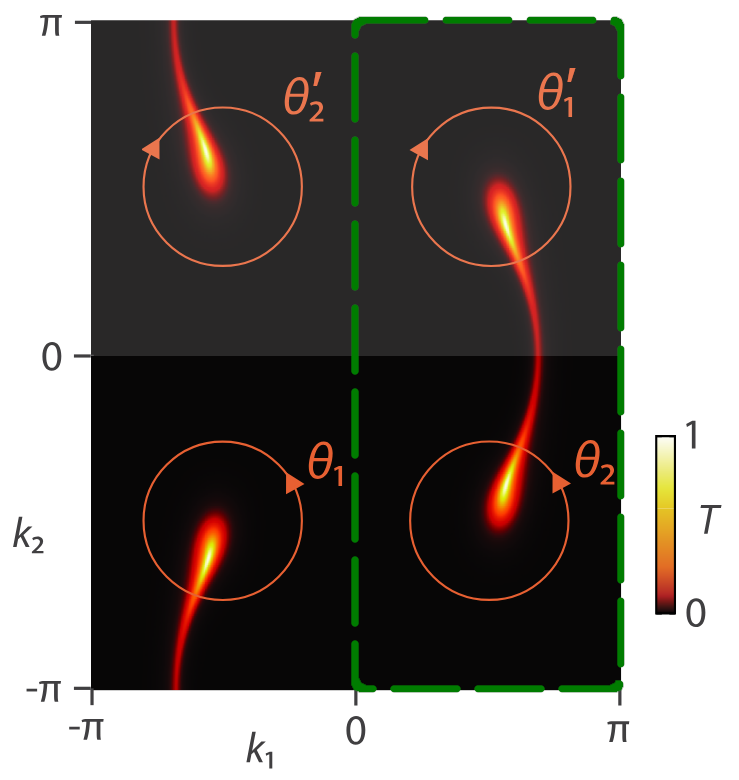
\includegraphics[width=.5\linewidth]{Images/K2-experiment-alt}
	\caption{Figure adapted from Ref.~\cite{Fonseca-Vaidya_nonorientable}, depicting the same system as Figure~\ref{fig:K2-experiment}. The lower black region is the $K^2$-like fundamental domain used by the authors. The upper grey region is obtained by mirroring this domain horizontally, completing the surface Brillouin torus. The two circular integration domains parametrised by $\theta_1$ and $\theta_2$ are mirrored to oppositely oriented circles parametrised by $\theta_1'$ and $\theta_2'$ respectively. Because the system respects this symmetry, the clockwise dispersion along $\theta_1'$ and $\theta_2'$ will look identical to the counter-clockwise dispersion along $\theta_1$ and $\theta_2$. In other words, if the contour around the upper points is taken along the more conventional counter-clockwise direction, the dispersion is mirrored with respect the lower points (i.e.\ it descends from the conduction band to the valence band instead of ascending as it does in Figure~\ref{fig:K2-experiment}). As a result, the fundamental domain chosen as in Figure~\ref{subfig:BZ_right} (here outlined in green) features two oppositely charged points with conventional dispersion characteristics.}
	\label{fig:K2-experiment-alt}
\end{figure}

The surface states obtained by truncating the system in the $x$ and $y$ directions cannot quite as readily be expressed in terms of a similar surface Mayer--Vietoris sequence. For example, an straightforward projection in the $k_x$ direction loses information about the $k_x\leftrightarrow-k_x$ action of the glide symmetry. One result of this is that the surface Brillouin zone is orientable in this direction---it has the topology of the 2-torus $\T^2$, and the glide symmetry reduces to a half lattice translation. Still, this symmetry appears to reverse the orientation of the surface Weyl points and their associated Fermi arcs; see Figure~\ref{fig:BZ_yz-surface}.
\begin{figure}[htb!]
	\centering
	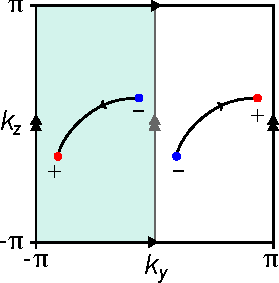
\includegraphics[width=.45\linewidth]{Images/BZ_yz-surface}
	\caption{Surface Brillouin zone in the $yz$ direction, with the projected fundamental domain indicated in teal and a possible configuration of Fermi arcs. This surface features an orientation-preserving translation symmetry in the $k_y$ direction. This symmetry still reverses both the chirality of the projected Weyl points (which is not expected under an orientation-preserving symmetry) and the orientation of the Fermi arc, appearing to indicate that both the cohomology and the homology must be twisted.}
	\label{fig:BZ_yz-surface}
\end{figure}
This seemingly tells us that the coefficients of both the homology and cohomology should be twisted. This seems to disagree with Equations~\eqref{eq:twisted-hom-duality} and \eqref{eq:twisted-cohom-duality}, but in reality, those relations specifically hold for twists which respect the orientation of the manifold. In general, simultaneous twists in the homology and cohomology are permitted, as long as the \emph{relative} twist between the coefficients respects the orientation. In this case, then, the correct description might be constructed in terms of twisted homology and cohomology, where the coefficients are twisted in such a way that they change sign under the $k_y\mapsto k_y+\pi$ symmetry. There may even be a canonical way to induce this twist from the projection $\pi_x$, based on the action of the glide reflection in the $k_x$ direction. These ideas certainly deserve further thought; for one thing, it becomes necessary to calculate the twisted groups without resorting to an ordinary Poincaré dual group.\footnote{
	The application of different twisted groups to topological matter has been studied in some detail in the more abstract setting of K-theory \cite{FreedMoore_K-theory,Thiang_K-theory}. The cohomology setting that we are working in is essentially a more tractable specialised version of this.}

The projection in the $k_y$ direction comes with challenges of its own, owing to the fact that the half lattice translation is projected out. The resulting surface of the Brillouin torus is mirror symmetric, and from its perspective, it appears as though the surface could host a single pair of Weyl points connected by a symmetric Fermi arc. In reality, such a configuration would require double charges to be physical, resulting from the projection of a configuration such as that in Figure~\ref{fig:double-points}. Tentatively, this may indicate that the pushforward of the projection $\pi_y$ simply isn't surjective, and attempting to calculate (co)homology groups on this surface may fundamentally ``overclassify'' the possible topology.


\markedsection{Brillouin zones}{Other non-orientable Brillouin zones} \label{sec:non-ori_classification}

As we have reviewed in Sections~\ref{sec:review} and \ref{sec:clarifications}, the fact that a single glide symmetry has a free action on the Brillouin torus does not guarantee that a combination of multiple glide symmetries also acts freely. This raises the question of whether there are any other momentum space symmetries besides the single glide reflection which give rise to a proper non-orientable fundamental Brillouin zone without high-symmetry points. Indeed, there are several in three dimensions; the aim of this section is to provide a complete overview of these symmetries. 

We also provide a cohomological classification of the insulator and Weyl semimetal invariants existing on these three-dimensional non-orientable Brillouin zones, under the assumption that the symmetry has its usual unitary action on the Hamiltonian. That is, we present the invariants obtained from ordinary cohomology and twisted homology, similar to the $\KS$ case discussed in the previous section. All explicitly calculated cohomology groups in this section are obtained using cellular homology.

In order to ensure completeness, the classification of fundamental Brillouin zones must rely on the theory of \emph{space groups}, which fully categorise the possible symmetry operations on periodic systems \cite{ITC_A}. We begin by briefly reviewing the two-dimensional case.

In two dimensions, the situation is quite manageable: there are only 17 space groups in total, which are referred to as the \emph{wallpaper groups}. Of these, 13 are symmorphic, meaning their generators are symmetries with fixed points (i.e. mirror reflections and rotations in 2D). As a result, these groups cannot have a non-trivial free action. The four remaining non-symmorphic groups include at least one glide symmetry. Of these, it turns out that only the wallpaper group $pg$ featuring a single glide symmetry has a free action \cite{Michel_crystal-symmetry}. This is precisely the symmetry that gives rise to the Klein bottle shaped fundamental domain first discussed in Ref.~\cite{CYZ_Klein-gauge}. We conclude that the Klein bottle $K^2$ is the only non-orientable two-dimensional manifold that can act as the Brillouin zone of a crystalline system.\footnote{
	Again, this related to the fact that it is the only non-orientable manifold with a vanishing Euler characteristic.}
We have already studied its topology as a surface Brillouin zone in Equation~\eqref{eq:K2-MV-explicit}.

In three dimensions, there are a total of 230 space groups. Among these, 73 are symmorphic (i.e.\ generated by point-fixing symmetries such as inversion, reflection and rotation) and the remaining 157 are non-symmorphic, featuring at least one glide reflection or screw rotation---the latter being a combination of a rotation and fractional lattice translation. Of the non-symmorphic space groups, a total of 12 have a group action that is free \parencite[Eq. (110)]{Michel_crystal-symmetry}. Of these, eight are generated only by screw rotations, which are orientation-preserving---just like ordinary rotations. This means they give rise to orientable fundamental domains, which can be classified using ordinary homology and cohomology. Nevertheless, these orientable Brillouin zones may feature non-orientable subspaces giving rise to $\Z_2$ invariants. Furthermore, we will discuss instances in which screw rotations are combined with glide reflections. For these reasons, we briefly expand on one of these space groups here before moving on to the four orientation-reversing cases.

The simplest space group featuring a screw rotation is $P2_1$, which is a $\Z_2$ group generated by a combined half turn and half lattice translation. For example, taking the screw axis to be the $y$ axis, a Hamiltonian with momentum space $P2_1$ symmetry obeys the relation
\begin{equation*}
	\Hc(k_x, k_y, k_z) = U\Hc(-k_x, k_y+\pi, -k_z)U^{-1}.
\end{equation*}
The fundamental domain of this symmetry can be taken to be the half torus with $-\pi\leq k_y\leq0$ just as for the glide symmetry, but the boundary identifications are different: instead of mirroring the $k_y=-\pi$ face before identifying it with the $k_y=0$ face, it must be rotated by a half turn. The resulting Brillouin zone topology is dubbed a ``half-turn space'' in Ref.~\cite{Zhu_acoustic-Klein-halfturn}, which probes a system with such a momentum space symmetry experimentally.\footnote{
	To be precise, the full space group obeyed by the system in Ref.~\cite{Zhu_acoustic-Klein-halfturn} is $P2_1/c$, which also features a glide symmetry; the action of this space group is not free.}
The explicit semimetal Mayer--Vietoris sequence of this space is as follows:
\begin{equation}
	0 \to \Z\oplus\Z_2^2 \to \Z\oplus\Z_2^2\oplus\Z^{k-1} \to \Z^k \to \Z \to 0.
\end{equation}
That is, the insulating invariants on the half-turn space are classified by $\Z\oplus\Z_2^2$, and Weyl points in the fundamental domain obey the regular Nielsen--Ninomiya theorem. The two $\Z_2$ invariants stem from $K^2$-like subspaces of the half-turn space, one of which is illustrated in Figure~\ref{fig:Halfturn-K2}.
\begin{figure}[htb!]
	\centering
	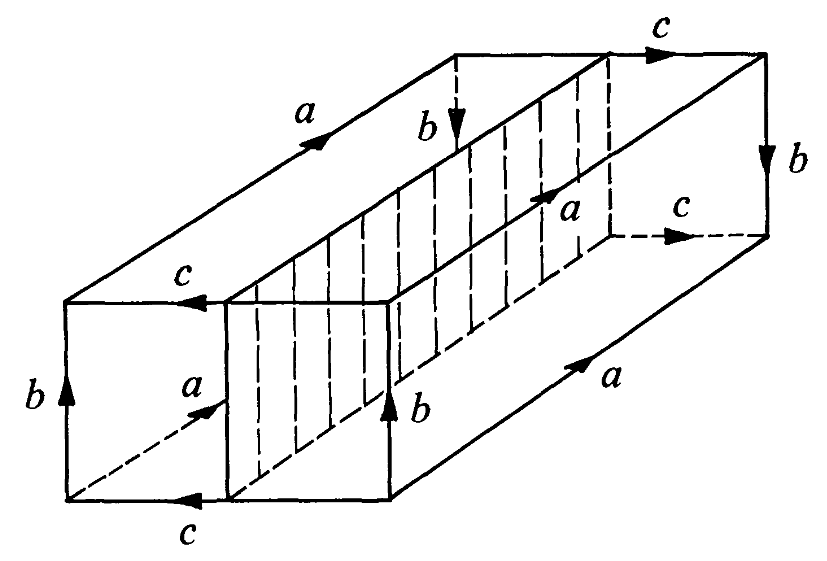
\includegraphics[width=.6\linewidth]{Images/Halfturn-K2}
	\caption{Figure from Ref.~\cite{Woll_One-sided}. The half-turn space (called a ``twisted cube'' in that work) is shown with a two-dimensional subspace, which has the topology of a Klein bottle.}
	\label{fig:Halfturn-K2}
\end{figure}

\subsubsection{Free orientation-reversing space groups in 3D}

We now turn our attention to the four remaining space groups with free actions, all of which give rise to a non-orientable Brillouin zone. The first and simplest of these is $Pc$, and it is precisely the $\Z_2$ group generated by a single glide symmetry that we have discussed at length in this chapter. Its semimetal Mayer--Vietoris sequence is given in Equation~\eqref{eq:explicit-sequence-nonorientable}, and we refer to Section~\ref{sec:invariants} for its interpretation.

The remaining three groups---$Cc$, $Pca2_1$ and $Pna2_1$---all combine a glide symmetry with another operation to form a $\Z_2\oplus\Z_2$ group. As such, the fundamental Brillouin zones that they induce cover exactly one fourth of the full Brillouin torus $\T^3$. Just as in the $\KS$ case, these fundamental domains can be parametrised in any number of ways, without changing the topology of the underlying manifolds. As such, we will remain agnostic about the choice of fundamental domain here, and simply provide the relevant Mayer--Vietoris sequences. The reader wishing to develop an intuition for the ways in which these spaces can be partitioned is referred to a space group atlas such as Ref.~\cite{Cockcroft_CD-ROM}.

The group $Cc$ combines a glide symmetry and a diagonal half-lattice translation, in such a way that the Hamiltonian obeys the following relations under momentum space $Cc$ symmetry (up to coordinate permutations):
\begin{align*}
	\Hc(k_x, k_y, k_z) &= U\Hc(k_x, -k_y, k_z+\pi)U^{-1}, \\
	\Hc(k_x, k_y, k_z) &= U\Hc(k_x+\pi, k_y+\pi, k_z)U^{-1}.
\end{align*}
The Mayer--Vietoris sequence associated with the non-orientable Brillouin zone under this symmetry is as follows:
\begin{equation}
	0 \to \Z\oplus\Z_2^2 \to \Z\oplus\Z_2^2\oplus\Z^k \to \Z^k \to \Z_2 \to 0.
\end{equation}
Again, this is the sequence in terms of ordinary cohomology or twisted homology.

The space group $Pca2_1$ features a glide reflection and a screw rotation. The momentum space $Pca2_1$ symmetry acts on the Hamiltonian in the following way:
\begin{align*}
	\Hc(k_x, k_y, k_z) &= U\Hc(k_x+\pi, -k_y, k_z)U^{-1}, \\
	\Hc(k_x, k_y, k_z) &= U\Hc(-k_x, -k_y, k_z+\pi)U^{-1}.
\end{align*}
The associated Mayer--Vietoris sequence of ordinary cohomology groups is then
\begin{equation}
	0 \to \Z_2^2 \to \Z_2^2\oplus\Z^k \to \Z^k \to \Z_2 \to 0.
\end{equation}

Finally, the group $Pna2_1$ is generated by similar operations as $Pca2_1$, but with the glide reflection plane offset from $k_y=0$ by $\pi/2$; the resulting action on the Hamiltonian is
\begin{align*}
	\Hc(k_x, k_y, k_z) &= U\Hc(k_x+\pi, \pi-k_y, k_z)U^{-1}, \\
	\Hc(k_x, k_y, k_z) &= U\Hc(-k_x, -k_y, k_z+\pi)U^{-1}.
\end{align*}
The semimetal Mayer--Vietoris sequence in ordinary cohomology is
\begin{equation*}
	0 \to \Z_4 \to \Z_4\oplus\Z^k \to \Z^k \to \Z_2 \to 0.
\end{equation*}

On the whole, all of these space groups share the same mod 2 charge cancellation seen on $\KS$, as is to be expected from the non-orientability of the underlying Brillouin zone. Incidentally, all three Mayer--Vietoris sequences feature different insulating invariants, which immediately confirms that the underlying manifold is different for each of these space groups (and also different from $\KS$). The insulating topology under $Pna2_1$ symmetry is especially interesting, being classified by a single $\Z_4$ invariant. Such invariants are fairly uncommon; for example, they do not appear in the tenfold way classification in Table~\ref{tbl:tenfold-way}. The derivation of an explicit expression and physical interpretation for this invariant is somewhat beyond the scope of this work, but a twisted homology argument similar to that provided in Figure~\ref{fig:K2S1_invariants} may provide intuitive insight.

We would be remiss not to mention Ref.~\cite{Shiozaki_AHSS} again in this context. Similar cellular decompositions are used in that work to arrive at a comprehensive K-theory classification of invariants related to space group symmetries. In comparison, the present calculations in terms of Mayer--Vietoris sequences may offer more specific insights into the structure of the semimetal invariants, and the dual twisted homology picture may prove invaluable in interpretation. Another nuance is that our classification stems from a two band model, whereas that in Ref.~\cite{Shiozaki_AHSS} is a many band scheme; in principle, this makes for a more general description, but it may also give rise to invariants that are not reflected in the transport properties of the material.


\markedsection{Inversion}{Inversion-symmetric semimetal topology}\label{sec:inversion}

In this final section, we turn our attention to a very important class of Weyl semimetals: those obeying inversion symmetry. As discussed in Section~\ref{sec:WSM-symmetries}, all Weyl semimetals must break either time-reversal or inversion symmetry. Those with broken time-reversal symmetries are called magnetic Weyl semimetals, and many of their prominent physical realisations are inversion-symmetric \cite{Liu_magnetic-WSM,Belopolski_magnetic-WSM,Morali_magnetic-WSM}. Here, we develop an ansatz for the classification of these systems, and demonstrate that the resulting Mayer--Vietoris sequence agrees precisely with their relevant features.

Recall that inversion symmetry acts on the momentum space Hamiltonian as
\begin{equation*}
	\Hc(\k) = U\Hc(-\k)U^{-1}.
\end{equation*}
That is, it induces the same symmetry on the Brillouin torus as time-reversal symmetry, but without complex conjugation on the Hamiltonian. The classification of time-reversal symmetric (class AII) Weyl semimetals was completed in Ref.~\cite{Thiang_equivariant}, and we have reviewed it in some detail in Section~\ref{sec:T-WSMs}. The description provided there relies on ordinary equivariant homology, and twisted equivariant cohomology relative to the set of time-reversal invariant momenta (TRIM). As previously explained in Section~\ref{sec:formalism}, the use of twisted cohomology can be motivated by noting that the symmetry is orientation-reversing, and that each Weyl node in the Brillouin torus has a symmetric partner which has the same chirality.

The same orientation-reversing symmetry is present under inversion symmetry. However, the lack of complex conjugation ensures that symmetric pairs of Weyl nodes have opposite chiralities instead of equal chiralities in this case. Using the same heuristic from Section~\ref{sec:formalism}, we find that a proper (co)homology classification of inversion-symmetric Weyl semimetals should rely on some form of twisted equivariant homology and ordinary equivariant cohomology. To the knowledge of the author, the use of twisted homology for classification of topological phases is novel to this work, and such a description has not yet been published. Nevertheless, the insulating case has been studied in some detail using different topological tools. Since any semimetal Mayer--Vietoris sequence also includes the insulating invariants of a system, we offer a brief review of these invariants for later comparison. We recommence our construction of the semimetal sequence in Section~\ref{sec:inversion-ansatz}; the eager reader may choose to skip straight there without loss of continuity.


\subsection{Existing insulating classifications}\label{sec:inversion-existing}

The two first and most detailed classifications of three-dimensional inversion-symmetric topological insulators were developed in parallel and published independently: Ref.~\cite{Hughes_inversion} in 2011 by Taylor Hughes, Emil Prodan and Andrei Bernevig, and Ref.~\cite{Turner_inversion} in 2012 by Ari Turner et al. The works differ somewhat in scope and methodology (the latter is more explicitly topological in nature, making use of homotopy theory on the space of Hamiltonians), but both treat essentially the same invariants and draw all the conclusions relevant to us. As such, we will treat them in tandem. Both works treat systems with an arbitrary number of bands, but for simplicity we will take the liberty of specialising their results to our preferred setting of a traceless two band model, where a single band is always occupied.

Two types of insulating invariants are distinguished under inversion symmetry. The first are three Chern numbers $C_{x,y,z}\in\Z$. These are the same Chern numbers that make up the $\Z^3$ Chern vector discussed in Section~\ref{sec:3D-Chern}. The second type of invariant is defined at each of the eight high-symmetry points in the Brillouin torus (i.e.\ the TRIM): since inversion is an order two operation squaring to 1, its eigenvalues on states at the invariant momenta must be $\pm1$. At each TRIM $\kappa$, the eigenvalue of the occupied state under inversion is a $\Z_2$ topological invariant $\zeta(\kappa)=\pm1$. It is shown in Ref.~\cite{Turner_inversion} that there are no other types of invariants, so that inversion-symmetric insulators are fully classified by three Chern numbers and eight $\Z_2$ invariants.

These eleven numbers are not independent; it is shown in both works that they are subject to certain internal relations, illustrated in Figure~\ref{fig:inversion-relations}.
\begin{figure}[htb!]
	\centering
	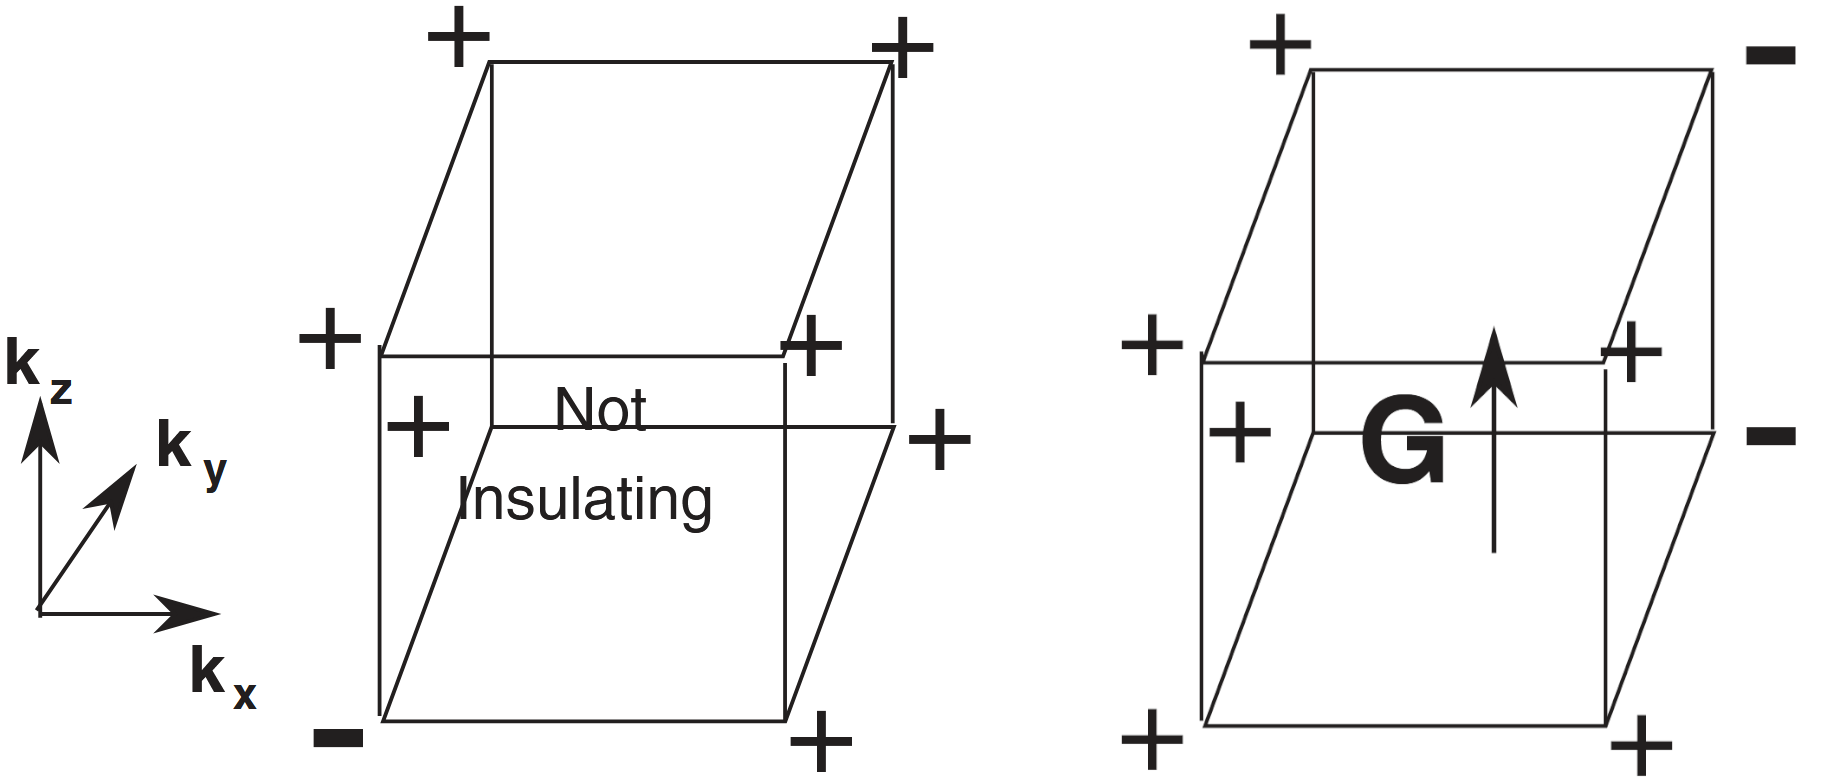
\includegraphics[width=.7\linewidth]{Images/inversion-relations}
	\caption{Figure from Ref.~\cite{Turner_inversion}. Each cube represents one eighth of the Brillouin torus, with the eight TRIM at the corners (e.g. $0\leq k_{x,y,z}\leq\pi$). Signs indicate the value of $\zeta$ at each TRIM. Left: an odd number of negative $\zeta$ indicates that the material is not an insulator, and must instead be a Weyl semimetal. Right: Both planes parallel to the $k_z$ axis feature odd numbers of negative $\zeta$, indicating that there is non-zero odd Chern number $C_z$.}
	\label{fig:inversion-relations}
\end{figure}
First of all, the product of all $\Z_2$ invariants must be positive in an insulator:
\begin{equation*}
	\prod_{\kappa\in\text{TRIM}} \zeta(\kappa) = 1.
\end{equation*}
In fact, it is argued in Ref.~\cite{Turner_inversion} that a value of -1 indicates that the material is a Weyl semimetal: at a TRIM $\kappa$, a negative value of $\zeta(\kappa)$ indicates that a Dirac string or loop passes through $\kappa$, and a closed inversion-symmetric Dirac loop must always pass through an even number of TRIM.

Secondly, the parity of each Chern number can be related to the product of $\zeta$ at four TRIM lying on a plane perpendicular to that Chern number's label: for example, $C_z$ is subject to the relation
\begin{equation*}
	\prod_{\kappa\in\text{TRIM}_{xy}}\zeta(\kappa) = (-1)^{C_z},
\end{equation*}
where TRIM$_{xy}$ denotes the set of TRIM lying on the $xy$-plane.

We note that the restrictions on the total product of signs and the three Chern number parities remove four $\Z_2$ degrees of freedom from three $C_{x,y,z}\in\Z$ and eight $\zeta(\kappa)\in\Z_2$, so that the effective group structure of the insulating invariants ends up being $\Z^3\oplus\Z_2^4$ instead of $\Z^3\oplus\Z_2^8$.\footnote{
	In a description with more occupied bands, the initial set of invariants is larger and this reduction is less dramatic as a result. However, even in this setting it is shown in Ref.~\cite{Turner_inversion} that for any given Chern number, there are 16 different classes of insulators with distinguishable transport properties. We note that this corresponds precisely to the 16 elements of $\Z_2^4$, which speaks in favour of the effectiveness of the two-band model.}
As a result, any semimetal Mayer--Vietoris sequence which we find must account for this $\Z^3\oplus\Z_2^4$ classification of insulating invariants.

As a final note before we return to our semimetal description, there have been several later papers which also identify certain invariants on inversion-symmetric systems using different methods: Refs.~\cite{LuLee_inversion,ShiozakiSato_order-two} use K-theory (which is closely related to cohomology) and Ref.~\cite{Khalaf_inversion} uses a construction in terms of layered lower dimensional systems. However, all these works give different invariants on 2D and 3D type A systems under inversion, and none of them straightforwardly accounts for both the $\Z$ and $\Z_2$ invariants present in the two-band model.

The latter observation might be taken to indicate a shortcoming of the two-band model. However, we note that a lot of the physical discussion in Ref.~\cite{Turner_inversion} appears to actually attest to its relative usefulness instead. This can be seen as follows: in the full $N$-band model discussed there, one is left with a $\Z^3\oplus\Z^8$ of invariants instead of the $\Z^3\oplus \Z_2^4$ derived above for the two-band model. It is then derived that for any given Chern number in $\Z^3$, there are 16 different equivalence classes among the remaining $\Z^8$ of insulators that have distinguishable transport properties. We note that this is in good agreement with the 16 elements of $\Z_2^4$, which appears to speak in favour of the physical effectiveness of the two-band model. In other words, while the full $\Z^3\oplus\Z^8$ of invariants are indeed all \emph{topologically} distinct, the two-band approximation may more naturally classify phases that are \emph{physically} distinct.


\subsection{Semimetal classification ansatz}\label{sec:inversion-ansatz}

We have already established that a (co)homology description of inversion-symmetric Weyl semimetals must rely on some form of ordinary equivariant cohomology and twisted equivariant homology. However, this does not tell us how the TRIM should be treated; for example, we have no information on whether the equivariant cohomology should be taken relative to the TRIM, excluding the TRIM, or as is without assigning the TRIM special status. In principle it should be possible to infer this information from careful mathematical study of the vector bundle structures that are induced by the symmetry. This precisely how the use of twisted equivariant cohomology relative to the TRIM is motivated for the time-reversal symmetric case in Ref.~\cite{Thiang_equivariant}, based on extensive mathematical analysis in Refs.~\cite{NittisGomi_Quaternionic,NittisGomi_FKMM}.

Instead of going to great lengths to perform such analysis, we will take a much more ad hoc approach: we develop an ansatz through some mathematical hand waving, and then show that this yields the correct invariants. The reasoning is as follows: in the cases of a free $\Z_2$ action that we have seen before, the effective Brillouin zone takes on precisely the topology of the quotient space $\T^3/\Z_2$---for example, the $\KS$ space that we have studied extensively---and this allows the equivariant (co)homology on $\T^3$ to be reduced to their more computable ordinary counterparts. Under the present $\Z_2$ inversion symmetry, the effective Brillouin zone [i.e.\ the half torus with the identifications pictured in Figure~\ref{subfig:TRS_orientation}] has the topology of $\T^3/\Z_2$ ``almost everywhere'': only the eight TRIM do not act as the quotient of two separate points in $\T^3$. The idea is now that we may still be able to use ordinary (co)homology on the effective Brillouin zone, as long as we can find a consistent and unambiguous way to make sense of the behaviour at the TRIM.

As was the case with the interpretation of the insulating invariants on $\KS$ in Section~\ref{sec:invariants}, the best intuition for this scheme is afforded by the twisted homology picture. In particular, it becomes apparent that the TRIM can act as endpoints of twisted Dirac strings from the perspective of the effective Brillouin zone; this is illustrated in Figure~\ref{fig:inversion_Dirac-strings}.
\begin{figure}[htb!]
	\centering
	\subcaptionbox{\label{subfig:inversion_four}}{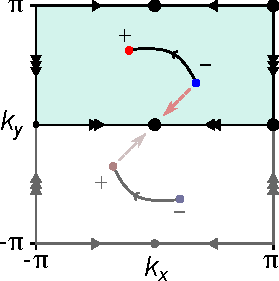
\includegraphics[width=.3\linewidth]{Images/inversion_four}}
	\hfil
	\subcaptionbox{\label{subfig:inversion_two}}{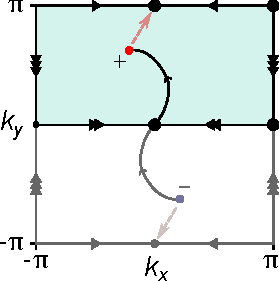
\includegraphics[width=.3\linewidth]{Images/inversion_two}}
	\hfil
	\subcaptionbox{\label{subfig:inversion_zero}}{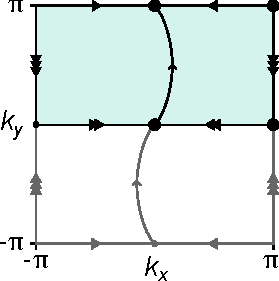
\includegraphics[width=.3\linewidth]{Images/inversion_zero}}
	\caption{A slice of the inversion symmetric Brillouin torus at $k_z=0$. The (arbitrarily chosen) effective Brillouin zone $M$ is shaded in teal, the four TRIM in this plane are indicated with big dots, and arrows indicate the correct boundary identifications. From left to right, a process of Weyl point annihilation is played out on the torus, while the apparent topology of (twisted) Dirac strings and loops is studied in isolation within $M$; the area outside of $M$ is greyed out as a reminder of this. (a) At first, the Dirac string contained within $M$ looks like a ``normal'' element of $H_1(M,W;\ext{\Z})$. The negative Weyl point in $M$ and its symmetric partner can be brought together along the orange arrows and annihilated at the TRIM at $\k=0$. (b) From the perspective of $M$, the TRIM at $\k=0$ seems to have absorbed the negative Weyl point, and the Dirac string appears to have a boundary at this TRIM as well as at the remaining Weyl point, meaning it looks like an element of $H_1(M,W\cup\text{TRIM};\ext{\Z})$. The remaining two Weyl points on the torus can be brought towards the TRIM at $\k=(0,\pm\pi,0)$ to annihilate. (c) After this final annihilation, the resulting Dirac loop looks like it runs between two different TRIM inside $M$, i.e.\ it looks like an element of $H_1(M,\text{TRIM};\ext{\Z})$.}
	\label{fig:inversion_Dirac-strings}
\end{figure}
In the same way that homology relative to the set of Weyl points $W$ encodes endpoints of Dirac strings, we propose that the correct effective description on the effective Brillouin zone $M$ is that of twisted homology relative to the TRIM. Explicitly, the twisted homology sequence in Equation~\eqref{eq:homology-sequence-nonorientable} then becomes\footnote{
	One might expect the third group in this sequence to become either $H_0(W,\text{TRIM};\ext{\Z})$ or (given the boundary map before it) $H_0(W\cup\text{TRIM};\ext{\Z})$. In fact, both are isomorphic to $H_0(W;\ext{\Z})$. The former directly so because there are no TRIM in the set $W$; the latter is a consequence of the twist in the coefficients, which ensures that $H_0(\text{TRIM};\ext{\Z}) = -H_0(\text{TRIM};\ext{\Z}) = 0$ under the action of the symmetry.}
\begin{align*}
	0\ &\to\ H_1(M, \text{TRIM}; \ext{\Z})\ \to\ H_1(M, W\cup\text{TRIM}; \ext{\Z})\ \\
	&\quad \overset{\partial}{\to}\ H_0(W;\ext{\Z})\ \to\ H_0(M, \text{TRIM}; \ext{\Z})\ \to\ 0.
\end{align*}

This sequence can be turned into a semimetal Mayer--Vietoris sequence in cohomology, using a twisted version of the modified Poincaré duality in Equation~\eqref{eq:semimetal-duality}. This duality tells us that the cohomology must be must be taken \emph{excluding} the TRIM rather than relative to it:
\begin{align*}
	0\ &\to\ H^2\big(M\setminus\text{TRIM}\big)\ \to\ H^2\big(M\setminus W\cup\text{TRIM}\big)\ \\
	&\quad\to\ \bigoplus_{w\in W} H^2(S_w^2)\ \to\ H^3\big(M\setminus\text{TRIM}\big)\ \to\ 0.
\end{align*}
This exclusion of the TRIM has an interesting side effect: it ensures that the action of inversion symmetry is completely free on the remaining space, so that the groups in this sequence are fully equivalent to the equivariant cohomology which we are trying to emulate.

Now that we have reduced our tentative invariant groups to untwisted, non-equivariant cohomology, they may once again be calculated using basic cellular homology. The removal of the TRIM makes this calculation somewhat more cumbersome than the others appearing in this chapter,\footnote{
	To be specific, $M$ is no longer closed after removing the TRIM. In order to find a cell structure, one can ``grow'' the holes in the space while maintaining the correct boundary identifications, until only a set of surfaces remains (in technical terms, one can deformation retract $M$ onto a 2-skeleton). The resulting cell structure is relatively complex, so that extracting its homology takes some work. This work can be facilitated using a computational tool such as the Smith normal form \cite{Peltier_Homology-computation}.} %TODO appendix?
but the conceptual basis is still relatively simple. The explicit semimetal Mayer--Vietoris we obtain in this way is as follows:\footnote{
	The $\Z_2^4$ components stem from $H_1(M\setminus\text{TRIM})\cong\Z_2^4$. Interestingly, this is essentially equivalent to the equivariant homology calculation that is performed in Ref.~\cite{Thiang_equivariant} to obtain the four $\Z_2$ invariants under time reversal: both groups end up classifying T-stable loops on the torus that avoid the TRIM.}
\begin{equation}\label{eq:inversion-MV-explicit}
	0 \to \Z^3\oplus\Z_2^4 \to \Z^3\oplus\Z_2^4\oplus\Z^r \to \Z^r \to 0 \to 0,
\end{equation}
where $r$ is the number of Weyl points in the fundamental domain, i.e.\ there are 2$r$ Weyl points on the full torus $\T^3$.

There are two features of this sequence that stand out immediately. The first is that the insulating invariant group on the left precisely matches the $\Z^3\oplus\Z_2^4$ derived from the literature in Section~\ref{sec:inversion-existing}. The second is the appearance of a trivial 0 group on the right, as opposed to the $\Z$ or $\Z_2$ we have seen in other contexts. This implies that there is no notion of charge cancellation at all on the effective Brillouin zone, i.e. the total Weyl point charge contained in it can take on any integer value. This agrees exactly with the existence of states such as the one pictured in Figure~\ref{subfig:inversion_two}, which feature only single Weyl point of charge $\pm1$ in the effective Brillouin zone; any number of such states can be stacked in order to obtain different total net chiralities.

We should reiterate in this context that the lack of charge cancellation that arises in the mathematical description is not reflective of a physical anomaly of any sort. Rather, not unlike on $\KS$ and other cases we have seen, it results from the fact that each Weyl point comes with its own charge cancelling partner. This is perhaps easier to accept for the system under consideration here; inversion symmetric Weyl semimetals are exceedingly well studied from a physical point of view, and to the knowledge of the author, this non-standard charge cancellation is never a real consideration. One simply studies the behaviour of the material across the entire Brillouin torus, where no such issues arise. Arguably, the situation is somewhat different from $\KS$ because the lack of a free group action implies that the Brillouin zone cannot truly be reduced to a fundamental domain, but for all physical intents and purposes, this changes little about the interpretation of features like charge cancellation. We maintain that even for systems like the single glide symmetry, the most natural setting to study phenomenological features is the complete Brillouin torus.

For completeness, we offer a basis of the insulating invariant group
\begin{equation}\label{eq:inversion-insulating}
	H_1(M, \text{TRIM}; \ext{\Z}) \cong \Z^3\oplus\Z_2^4
\end{equation}
in terms of twisted Dirac loops, just as we did in Figure~\ref{fig:K2S1_invariants} for the $\Z\oplus\Z_2$ that generates the two invariants on $\KS$. There, we represented the twisted Dirac loops on $\KS$ by glide symmetric sets of loops on the whole torus $\T^3$; we will proceed similarly here by considering inversion symmetric loops on the torus. To this end, we introduce some notation. Taking Figure~\ref{subfig:inversion_zero} as an example, it depicts the loop on the torus that runs through the two TRIM at $\k=0$ and $\k=(0,\pi,0)$ in the positive $k_y$ direction. This loop is inversion symmetric, and we denote it by $\ell_{0y0}$. Had the loop run up through $\k=(\pi,0,0)$ and $\k=(\pi,\pi,0)$, we would notate $\ell_{\pi y0}$ instead. Similarly, the loop $\ell_{x0\pi}$ runs through $\k=(0,0,\pi)$ and $\k=(\pi,0,\pi)$ in the positive $k_x$ direction, those representing $\ell_{\pi\pi z}$ run through $\k=(\pi,\pi,0)$ and $\k=(\pi,\pi,\pi)$ with increasing $k_z$, and so on. There are twelve of these loops in total: four for each coordinate direction.

These loops have a key property that allows them to generate the group in Equation~\eqref{eq:inversion-insulating}: while they cannot individually be detached from the TRIM that they run through without breaking inversion symmetry, they can be once they are doubled up; see Figure~\ref{subfig:inversion_detach}.
\begin{figure}[htb!]
	\centering
	\subcaptionbox{\label{subfig:inversion_detach}}{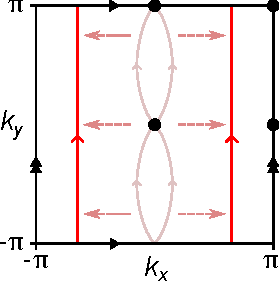
\includegraphics[width=.35\linewidth]{Images/inversion_detach}}
	\hfil
	\subcaptionbox{\label{subfig:inversion_equiv}}{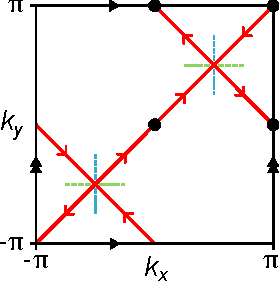
\includegraphics[width=.35\linewidth]{Images/inversion_equiv}}
	\caption{(a) Two copies of $\ell_{0y0}$ can be moved apart in opposite directions while respecting inversion symmetry. Moving the loops even further apart makes them intersect the TRIM at $k_x=\pi$ simultaneously, proving that in terms of twisted homology classes, $2[\ell_{0y0}] = 2[\ell_{\pi y0}]$. (b) Intermediate state between $\ell_{0y0} - \ell_{\pi y0}$ and $\ell_{x00} - \ell_{x\pi0}$. Detaching the intersections along the vertical blue dashed lines (as though cutting them with scissors) yields $\ell_{0y0} - \ell_{\pi y0}$, whereas cutting along the horizontal green lines gives $\ell_{x00} - \ell_{x\pi0}$.}
	\label{fig:inversion_relations}
\end{figure}
In this way it can be shown that $2\ell_{0y0}$ has the same twisted homology class as $2\ell_{\pi y0}$. This means the classes $[\ell_{0y0}]$ and $[\ell_{\pi y0}]$ cannot generate independent $\Z$ invariants. Instead, their difference must be a $\Z_2$ invariant:
\begin{equation*}
	2[\ell_{0y0}] = 2[\ell_{\pi y0}] \implies 2 [\ell_{0y0} - \ell_{\pi y0}] = 0.
\end{equation*}
Furthermore, it can be shown that $[\ell_{0y0} - \ell_{\pi y0}] = [\ell_{x00} - \ell_{x\pi0}]$; this is illustrated in Figure~\ref{subfig:inversion_equiv}. Using these and other similar relations, we find that the invariant group in Equation~\eqref{eq:inversion-insulating} is generated by the three $\Z$ generators
\begin{equation*}
	\nu_x := [\ell_{x00}],\quad \nu_y := [\ell_{0y0}],\quad \nu_z := [\ell_{00z}],
\end{equation*}
and four $\Z_2$ generators
\begin{equation*}
\begin{split}
	\nu_{xy} &:= [\ell_{x00} - \ell_{x\pi0}] = [\ell_{0y0} - \ell_{\pi y0}], \\
	\nu_{yz} &:= [\ell_{0y0} - \ell_{0y\pi}] = [\ell_{00z} - \ell_{0\pi z}], \\
	\nu_{xz} &:= [\ell_{00z} - \ell_{\pi0z}] = [\ell_{x00} - \ell_{x0\pi}],
\end{split}\qquad
\begin{split}
	\nu_{xyz} &:= [\ell_{x00} - \ell_{x\pi0} - \ell_{x0\pi} + \ell_{x\pi\pi}] \\
		&= [\ell_{0y0} - \ell_{\pi y0} - \ell_{0y\pi} + \ell_{\pi y\pi}] \\
		&= [\ell_{00z} - \ell_{\pi0z} - \ell_{0\pi z} + \ell_{\pi\pi z}].
\end{split}
\end{equation*}
We can translate directly between these twisted homology invariants and the invariants discussed in Section~\ref{sec:inversion-existing}, namely the three Chern numbers $C_{x,y,z}$ and eight inversion eigenvalues $\zeta(\kappa)$ at the TRIM $\kappa$. First, note that the $\Z$ generators all induce a Chern number of 1 in their respective directions, while the $\Z_2$ generators all have a zero Chern vector due to the loops running in opposite directions. This implies that the Chern vector is precisely indexed by the $\Z^3$ subgroup of the twisted homology.

The inversion eigenvalues $\zeta$ can be inferred by checking which TRIM are crossed by the loops in each of the generators: such crossings induce a sign change in the inversion eigenvalue. For example, each copy of $\nu_x$ changes the sign of $\zeta$ for the two TRIM on the $x$ axis, $\nu_{yz}$ affects the four TRIM on the $yz$-plane, and $\nu_{xyz}$ inverts the sign of $\zeta$ at all eight TRIM simultaneously. The total set of invariants can then be deduced from the combination of these actions. For instance, a topological state with twisted homology class $2\nu_x - \nu_y + \nu_{yz}$ has a Chern vector of $\vb{C}=(2,-1,0)$ and negative inversion eigenvalues only at the two TRIM $\k=(0,0,\pi)$ and $\k=(0,\pi,\pi)$.

Finally, the construction of all twisted Dirac string configurations, which exist in
\begin{equation*}
	H_1(M, W\cup\text{TRIM};\ext{\Z}) \cong \Z^3\oplus\Z_2^4\oplus\Z^r,
\end{equation*}
proceeds more or less the same as in Ref.~\cite{Mathai_math-review}: any given charge configuration on the set $W$ of Weyl points in the effective Brillouin zone fixes a unique element in the summand $\Z^r$. There then remain $\Z^3\oplus\Z_2^4$ different twisted Dirac string configurations, which are precisely generated by the action of the insulating group. To be precise, there is no canonical ``zero'' configuration, so one needs to fix a reference configuration and then obtain all other configurations by adding twisted Dirac loops from $\Z^3\oplus\Z_2^4$. It should be noted that this choice of a reference configuration means that the $\Z^3\oplus\Z_2^4$ subgroup does not correspond to the Chern numbers and inversion eigenvalues in the same canonical way as before. However, the inversion eigenvalues can still be obtained from the twisted Dirac strings by inspection: each TRIM $\kappa$ that is crossed by a Dirac string has $\zeta(\kappa)=-1$.

All in all, our heuristic approach to describing the invariants for this system has yielded a classification that appears highly plausible, in that all its major features agree with the properties of the system. Not only does this offer a useful platform for studying the semimetal invariants of this system directly, but it also demonstrates again the usefulness of the twisted homology point of view, and serves as a jumping off point for the classification of other symmetries featuring high-symmetry points. It also shows that the need for fully rigorous mathematical descriptions in terms of vector bundle classification can be bypassed based on more direct reasoning, at least in some cases. There is unquestionable value in these more rigorous methods, but it is often the more direct approaches which afford the greatest intuition---a quality that can be invaluable in developing proper physical understanding.